%% $RCSfile: proj_report_outline.tex,v $
%% $Revision: 1.2 $
%% $Date: 2010/04/23 02:40:16 $
%% $Author: kevin $

\documentclass[11pt
              , a4paper
              , twoside
              , openright
              ]{report}

\usepackage{float} % lets you have non-floating floats
\usepackage{wrapfig}

\usepackage{amsmath}
\usepackage{epigraph}
\usepackage{tikz}

\usepackage{url} % for typesetting urls

%
%  We don't want figures to float so we define
%
\newfloat{fig}{thp}{lof}[chapter]
\floatname{fig}{Figure}

%% These are standard LaTeX definitions for the document
%%
\title{Richer, Restricted Boltzmann Machines}
\author{Max Godfrey}

%% This file can be used for creating a wide range of reports
%%  across various Schools
%%
%% Set up some things, mostly for the front page, for your specific document
%
% Current options are:
% [ecs|msor]              Which school you are in.
%
% [bschonscomp|mcompsci]  Which degree you are doing
%                          You can also specify any other degree by name
%                          (see below)
% [font|image]            Use a font or an image for the VUW logo
%                          The font option will only work on ECS systems
%
\usepackage[image,ecs]{vuwproject}
\otherdegree{Bachelor of Engineering with Honours}

% You should specifiy your supervisor here with
%     \supervisor{Firstname Lastname}
% use \supervisors if there is more than one supervisor
\supervisor{Marcus Frean}

% Unless you've used the bschonscomp or mcompsci
%  options above use
%   \otherdegree{OTHER DEGREE OR DIPLOMA NAME}
% here to specify degree

% Comment this out if you want the date printed.
\date{}

\begin{document}


% Make the page numbering roman, until after the contents, etc/Users/Max/Downloads/honoursreport 2/content.tex.
\frontmatter

%%%%%%%%%%%%%%%%%%%%%%%%%%%%%%%%%%%%%%%%%%%%%%%%%%%%%%%

%%%%%%%%%%%%%%%%%%%%%%%%%%%%%%%%%%%%%%%%%%%%%%%%%%%%%%%

\begin{abstract}

In machine learning encoding prior knowlegde about a task can be essential to the technqiues ability to perform well on said task.(Big mental leap here....) This report explores and evaluates a novel approach to modelling data that is caused by two, independant sources. The theory has been proposed by Frean, Marcus and Marsland, Stephen, leveraging the popular Restricted Boltzmann Machine as a model for a source and a Sigmoid Belief Network as the way for these complex causes to combine. A new algorithm is presented under the dynamics of this model that allow indepedant representations of multi-cause data to be represented given a multi-cause input.

\end{abstract}

%%%%%%%%%%%%%%%%%%%%%%%%%%%%%%%%%%%%%%%%%%%%%%%%%%%%%%%
\maketitle

%\chapter*{Acknowledgments}\label{C:ack}
I would like to thank my supervisor Marcus Frean for the constant support and
mentorship throughout the year. Also for teaching me so much, and the opportunity to
work on something so neat. I would also like to
thank Stephen Marsland, co-inceptor of the idea for this project.



\tableofcontents

% we want a list of the figures we defined
%\listof{fig}{Figures}

%%%%%%%%%%%%%%%%%%%%%%%%%%%%%%%%%%%%%%%%%%%%%%%%%%%%%%%
\mainmatter
%%%%%%%%%%%%%%%%%%%%%%%%%%%%%%%%%%%%%%%%%%%%%%%%%%%%

% individual chapters included here



\chapter{Introduction}

\section{Problem}
\subsection{Deep Belief Networks can achieve state of the art performance}
% Deep beleif networks are the shit
  % Proven good for images and speech, text analysis (sentimenet analysis)
Deep Belief networks are powerful models that have proven to achieve state of the art performance in many domains. For instance a non-exhaustive list is image classification, dimensionality reduction, natural language recognition, Document classification, Semantic Analysis and .

% Captures deep interactions between complex features. In image domain this is the relationships between pixels.
  % e.g. in an image at best low level layers learn images filters
DBNs capture non-linear interactions between low level features, in the context of image classification the lower layers should capture image filters.

\subsection{DBNs have no mechanism for separating sources}
% Deep belief networks have no way to separate the sources.
Despite a DBNs expressiveness, their is no way to extract these interactions. If an input has multiple sources then the complex combination is instead learnt, the network has no mechanism for extracting multiple causes.
% This is the motivation for this project, we want a way to separate, and model the sources of input data, where said data is a complex combindation of two sources acting independantly.
This is the motivation for this project, to be able to separate the sources of data in a new model.

 \cite{2015HistSciPy}

% Deep Belief Networks are constructed by stacking Restricted Boltzmann Machines (RBMs). This proved a natural starting point for representing two sources. We worked in a shallow environment before attempting to stack RBMs.
\subsection{Restricted Boltzmann Machines cannot separate sources either}
Restricted Boltzmann Machines are two layer, fully connected, unsupervised nueral networks. DBNs are constructed by stacking RBMs. Being the building block of the powerful DBN, RBMs are a natural starting point for representing mutliple sources.
% RBMs make a strong assumption that all features are dependant in the prior, inheriently modelling a single source.
RBMs make the assumption that the features of the input data are dependant in the prior, as they are independant in the posterior. The latter makes them tractable to use in practice, but also means they model/encode a single representation.
  % In the image domain, this equates to all pixels being assumed relevant to what we are trying to model. With enough examples RBMs can generalise, but there is no mechanism for modelling independant subjects.
  Again using the example of images, an input image will map to a single representation, again there is a lack of mechanism for modelling sources that are acting independantly.

% There is another structure, Belief/Bayesian Networks, and the parameterised version, the Sigmoid Belief Network, which makes the polar assumption where each feature is modelled by an independant cause. These are intractable to train in practice.
\subsection{Sigmoid Belief Networks; Intractably rich in practice}
The Sigmoid Belief Network, the parameterized version of a Bayesain/Belief network appears as a natural choice for modelling inpendant sources in that it makes a polar assumption to the RBM; -- Warning Semicolon Use -- Every feature has an independant cause. The sigmoid belief networks assumption could capture data that has multiple sources, but this is intractable in practice.

% Frean, Marsland propose a generative model that aims for a middle ground between these two existing models.
\section{Solution}
\subsection{Trading tractibility for Source Separation}
Frean and Marsland propose a generative model that aims to trade a small amount of the RBMs performance for richness, finding a middle ground between the sigmoid beleif network and the restricted boltzmann machine.
Frean and Marsland also propose an algorithm to invert this model, seperating the sources of an input.

The new generative model, referred to onwards as an ORBM, uses an RBM to model each source and a sigmoid belief network to capture their combination to from data. This project explores the ORBM use for separating two causes.

\begin{figure}[h]
\begin{center}
  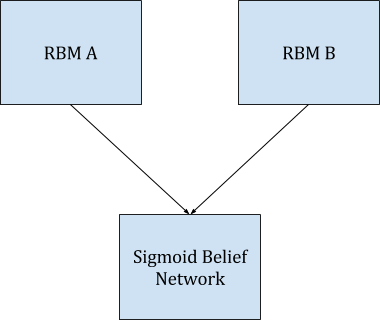
\includegraphics[width = 0.5\textwidth]{Assets/ORBM_fig_1}
\caption{The proposed generative model for capturing two causes, the ORBM.}

\label{F:ORBM-fig-1}
\end{center}
\end{figure}

Given the proposed model and algorithm, this project answers the following questions:
\begin{itemize}
  \item Can this model encode data comprised of more than one cause as it's constituted causes? That is, can the model and new algorithm for inverting it, perform source separation.
  \item Is the ORBMs two cause structure to rich to be tractible in practice?
\end{itemize}


% \chapter{Introduction}

\section{Problem}
(Could I just say models, here instead of generative models?)
\begin{itemize}
  \item Real world data if often causesed by multiple sources, that is independant sources combining to form data.  This creates noise and obscures part of the data we are interested in.
  \item Generative Models used in Machine learning do not capture these source independantly, meaning prior knowledge about the data is being lost(To much of a sweeping statement?). Instead the generative models are trained to learn the complex combination of data caused by the sources.
  \item Generative Model that do account for multiple sources are desirable, as the causes are encoded separately, which would(should this just be allows?) allow source separation. That is, taking a noisy input and encoding that into separate representations for each source.
  \item When the model treats sources naively, more work on data preprocessing and cleaning is needed, which often takes longer that the machine learning task itself.
  \item Frean, Marsland propose a new Generative Model that can capture two causes combining to form data, effectively encoding prior knowlege into the architecture of the model.
  \begin{itemize}
    \item It builds on and combines previous work on Restricted Boltzmann Machines and Sigmoid Belief Networks.
    \item The theory had been checked but the new model had not been tried in practice. Frean and Marsland needed confidence around some key areas
    \begin{itemize}
      \item Can this model encode a multi-cause input(need to define this?) as separate causes? That is, can the model be used to perform source separation. Given this produces an internal representation, how can we evaluate whether or not is it working?
      \item How does the time-efficiency of this model compare to the standard Restricted Boltzmann machine? The architecture of the new generative model has a richer structure. The theory shows that the new approach has the potential to be slower than an RBM to generate a hidden representation. Is this an issue in practice?
    \end{itemize}
    \item These are non-trivial tasks as the Restricted Boltzmann Machine, and the proposed model that uses it, are stochastic unsupervised learners making evaluation non-trivial. We cannot simply inspect the representations generated in the new model.
    \item There is(was?) a need to implement this new approach and then verify that it can or cannot perform source separation.
  \end{itemize}
  \item In addition to the new algorithm Two approximations that allow the algorithm
  more efficient need to be evaluated and compared to the full approximation.
\end{itemize}

\section{Solution}\label{Sec:Intro:Solution}

\begin{itemize}
  \item This project answered(answers?) these questions, evaluating the new generative model by way of experimentation. The ablility for the new generative model (I really need a name for this)  to separate the sources has been evaluated on various sizes (better word here) of problems.
  \item The unsupervised nature of the new model and the models it builds on, are non-trivial to evaluate. To explain the evaluation techniques and the new model itself some concepts/terminology must first be introduced.
\end{itemize}

\section{A Concrete Scope}

As the theory already had the Mathematical ground work by Frean and Marsland the scope of this project is not to prove the theory mathematically, instead impelmenting the Algorithm and verfiying how it behaves in practice by answering the questions posed in \ref{Sec:Intro:Solution}.

\chapter{Background}

\section{Context}

\subsection{Source Separation}

\begin{itemize}
  \item Introduce the idea of data with mutiple sources, probably by way of the cocktail party problem like in prelim.
  \item Go on to reference previous work in Source separation to show the importance/interest in the area. 5 Papers should suffice.
\end{itemize}

\subsection{Probablistic Graphical Models}

Probalistic Graphical Models or PGMs for short, are an expressive way to represent a collection of stochastic  variables. If the graph is directed then the edges represent causation, this is also referred to a Bayesian network. Conversely, if the graph was undirected then edges represent a mapping. TODO-CITE-DAVID-BARBERS-TEXTBOOK-ON-PGM-USE.

\subsection{Generative Models}

Generative models are a powerful way to model data. (TODO-GRAB-THOSE-GENERATIVE-MODEL-USES-CITATIONS)

In the context of images, generative models, if trained, can randomly generate observable data. (Don't like the wording of this)
The generative model proposed in this project aims to represent data generated by two causes.

  \subsubsection{Observable and Hidden Variables}

  \begin{itemize}
    \item Describe how the models have some latent factors/variables that represent the cause, or an efficient encoding/representation of the data we want to learn.
    \item Make sure to describe/define analogus terms like hidden visible layers, variables/units etc.
  \end{itemize}

  \subsubsection{Training Generative Models}
  \begin{itemize}
    \item Training generative models with some param big theta, gradient amounts to log likelihood of dataset minus normalisation.
    \item Amounts to hebbain learning. Reasoned about by Donald Hebb, connections between neurons in the brain during learning, the more often a memory is accessed or used, the strong the connection it should make. Nice to have parallels with biology. Something biology performs well that Machine learning has difficulty with is source separation.
    \item Wake phase - Often referred to as the clamped phase of training involves clamping the input of the model to a data item and trying to increase that items probability. Essentially this amounts to building probabilty mass around the items in the training set.
    \item Sleep phase - Also referred to as the free phase, this acts as complexity control where the the generative model is used to create data items...
    \item Quickly talk about the learning rule
  \end{itemize}

\subsection{Sampling}

Sampling is the process of drawing samples from a distribution. It is used when the distrubtion we want samples from is intractable to calculate analytically. Sampling is required to train generative models, as often the gradient to be climbed/descended involves calculating a probability in the
generative model.

\begin{itemize}
  \item Inference is the process of given reasoning about what we do not know given that of which we do know.
  \item In a Generative Model this amounts to the Posterior
\end{itemize}

  \subsubsection{Markov Chain}

  \begin{itemize}
    \item The importance of Markov Chains and mixing time are crutial in this project
  \end{itemize}


  \subsubsection{Gibbs Sampling}

  Gibbs sampling is a special case of Markov Chain Monte Carlo, a technique for sampling from a complex distribution. The probability mass of a generative model is a common use case for Gibbs sampling.

  \subsubsection{Reconstructions}

  Generative Models can create an internal representation given an input. They can also generate a faux input given an internal representation. Performing one Gibbs iteration, that is sampling from the hidden units given an input $ P(h|v) $ and then taking the generated hidden state and generating a faux input. The model tries to reconstruct the input.

  \subsubsection{Fanstasies of the Model}

  In the same way that a generative model uses reconstructions to try and recreate the      supplied input based purely on how it's represented that input, performing many, many (greater than 100) Gibbs iterations with no input pattern clamped allows the reconstructions to explore the probability mass that the model has built up during training. Sampling from these wanderings creates what are refferred to as 'fantasies' or 'dreams'. These give a sense of what the model has learnt, and can act a smoke test for if the model has actually capture anything.
  (TODO-CITE-PAPER-WITH-MNIST-DREAM-EVALUATION, they were crappy).

\section{An Intractable Model For Causes}
  \subsection{Belief Networks}

  A belief network is technique(? Graphical Network ?) of modeling causual data. The network is directed representing cause, nodes in the network represent binary variables which are dependant on ancestor nodes, the degree of which is encoded in a conditional probalitity table. The belief network provides a succint encoding of depedancies between variables. Several algorithms operate on this representation, determining the probability of a variables state, given the states of its ancestors. One of such algorithms is Belief Propagation/Sum-Product Algorithm. However this technique breaks down in larger dimensions with a cost of TODO


  The technique proposed in this report relies on the parameterised version of the belief network, the Sigmoid Belief Network. The sigmoid belief network is composed of sigmoid units, akin to that of a perceptron linear threshold unit. The weighted sum of the inputs to a variable in the system is passed through a sigmoid function, the weights capturing the dependance between a node and its ancestors.

  Belief Networks appear to be an intuitive way to model data in machine learning, as rich dependancies often present in real data can be expressed in its architecture. Unfortunately, due to the effect of explaining away, it is intractable to perform inference in a belief network which is needed required for training.

  \subsection{Explaining Away}

  The power of the belief network is also its weakness, a rich structure that models a system of interest inheriently has depedancies. In its minimal case explaining away can be seen in a 3 node network popularised by TODO-CITE-AI-A-MODERN-APPROACH-TODO. TODO-GRAPHIC

  In this network knowledge of the alarm creates a dependance between Burglar and Earthqaukes. For instance, say the Alarm has gone off and we know an earthquake has occurred, our belief in being burgaled decreases. The dependance in belief networks means that sampling from the network requires a longer Markov Chain to mix.

  In the context of images, where there may be upwards of 1000 observable values, all with different depedancies this is intractable.

\subsection{Boltzmann Machines}

A Boltzmann machine shares a few qualities with Belief Networks. Both are generative models, and variables/nodes have probabilities of being active/deactive based on neighbouring nodes. Unlike a Belief Network, a Boltzmann Machine is a undirected network meaning connections between nodes no longer encode causal information. Performing gibbs sampling appears trivial in a Boltzmann Machine, in that to find the probability of a given unit being active a weighted input to that node is passed through a sigmoid function. However, in practice the recurrent nature of Boltzmann Machines makes sampling intractable.

TODO-REFENCE-PAPER-OF-THIS The Boltzmann Machine was shown, given an unreasonable amount of time, to be able to perform better than the state of the art at the time.

\section{The Current Approach: A Strong assumption}

\subsection{Restricted Boltzmann Machines}

\todo%
Talk about how Gibbs sampling in RBMs allows us to approximately sample from the hidden (unknown/representation) given the visible (known/input data).
\todo%

Hinton TODO-REFERENCE-THE-PAPER proposed a restriction by way of assumption to the Boltzmann Machine that makes it tractable to sample from and therefore train. Boltzmann Machines of this architecture are referred to as Restricted Boltzmann Machines, or RBMs for short.

The assumption being that the observable and latent variables are independant respectively, enforcing a two layer, fully connected bipartide structure. The affect of this being that inference can be tractably computed as the latent variables no longer become dependant given the observed variables.

  \subsubsection{Tractable Training - Contrastive Divergence}
  Hinton TODO-CITE-CLASSIC-PAPER proposed Contrastive Divergence as a method for training RBMs efficiently. The algorithm leverages the now tractable wake phase because $P(h|v)$ is efficeint to compute. However the free or sleep phase required another restriction where the network is only left to its own dynamics can be limited to only one iteration and still perform well. TODO-CITE-CD-PAPER

The observed variables are often referred to as the visible units, and will be so forth in this report. The latent variables are often referred to as the hidden units, and will be so forth in this report. Therefore the Restricted Boltzmann machine transforms some visible unit into a hidden representation. These two layers of units can be thought of as vectors of binary values, referred to as $ v $ and $ h $ for visible and hidden layers respectively.

This restriction allows an efficient calculation of the Wake Phase of generative model learning, as the $ P(h|v) $ can be calculated as a simple weighted sum passed through a sigmoid followed by a bernouli trial where the probability of being $1$ is equal to the result of sigmoid.



\subsection{Deep Learning}

  \begin{itemize}
    \item Discuss deep learning as there are clear parallels to Deep Belief Networks and the new approach
    \item in paritcular how the deep networks have this process of freezing the weights and creating a sigmoid belief layer instead. There seem to be clear parallels between a deep network with one RBM to the ORBM.
  \end{itemize}

\begin{itemize}
  \item Unrolling the gibbs chain and we are in effect training an infinite depth sigmoid beleif net (TODO-REFERENCE-HINTONS-PAPER-HERE)
\end{itemize}

  \subsection{Inference}
  One of the reasons the Restricted Boltzmann Machine is effective in practice is inference can be performed efficiently. Inference being computing the posterior.

  \subsection{Evaluating Restricted Boltzmann Machines}

  \begin{itemize}
    \item Being unsupervised makes it difficult to evaluate RBMs. Often used as part of a deeper network, feature extractor, autoencoder
    \item Hinton Diagrams allow visualisation of hidden unit utlisation (TODO-SOME-SORT-OF-CITE). The weights out of a given hidden unit can be visualised in visible data space. The weights should exhibit some structure if they are being utlisied. This is a good smoke tests for non-tulised hidden units will look very similar to units with random initial weights.
    \begin{itemize}
      \item Small Cases
      \begin{itemize}
        \item In trivial cases an RBM can inspected analytically. Reconstructions of the dataset should match the dataset with approximately the correct proportion. For instance training RBMs on 2 bit XOR should result in mostly [1,0] and [0,1] but not [1,1] and [0,0].
        \item Hand craft weights can be used to perform inference in a 'perfect model'. For instance an RBM that can capture two bit, logical XOR can be represented as :TODO-INSERT-PIC
      \end{itemize}
      \item Large Cases
      \begin{itemize}
        \item In non-trivial cases, with larger datasets, reconstructions can be compared to the dataset but given the unsupervised nature of RBMs emperically detecting if a model is trained is difficult.
        \item The log liklihood of the RBMs generative model exbiting the dataset is a good measure that can be approximated (because we have to sample).
        \item We can train a classifier on the RBMs hidden representation. This can be compared for a ORBM and RBM.
      \end{itemize}
    \end{itemize}
  \end{itemize}

  \begin{figure}[]
  \begin{center}
  	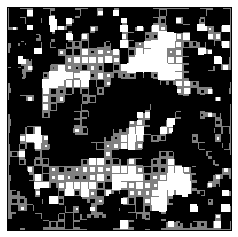
\includegraphics[]{Assets/HINTON1}
  \caption{ Good Hinton Diagram}
  \label{F:TEMP}
  \end{center}
  \end{figure}
  \begin{figure}[]
  \begin{center}
    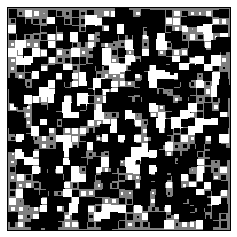
\includegraphics[]{Assets/HINTON2}
  \caption{Bad Hinton Diagram}
  \label{F:TEMP}
  \end{center}
  \end{figure}


  \section{A New Approach - The ORBM}

  \begin{itemize}
    \item Frean and Maslands new approach combines the Restricted Boltzmann Machine and the Sigmoid Belief Network, the RBMs allowing the rich complex causes to be encoded independantly, and the Sigmoid Belief Network modelling the combination of the causes to form the observable data.'
    \item By building on these existing methods can leverage exisitng algorithms
    \item Can verify the inference algorithm with pre trained RBMs for each cause.
    \item Like the RBM leveraged in the ORBM, it is difficult to evaluate, But similar techniques can be leveraged

  \end{itemsize}

  \subsection{Architecture}

  \begin{itemize}
      \item Two RBMs, on for each cause, then they combine via a Sigmoid Beleif Layer. Weights between the RBM and Sigmoid Layers are shared. (TODO-A-DIAGRAM)
      \item Diagram of the ORBM Architecture Including U Layer. Make sure I'm explaining the U layer.
      \item In fact Ua, Ub are like mirrors of the visible.
  \end{itemize}

  \subsection{Inference In the ORBM}

  The difference in architecture from an RBM means that a slightly different inference algorithm is required, as the representations are represented separately for a composite input.

  \begin{itemize}
    \item Inference in this generative model is P(ha, hb given v) , we want to represent the causes separately.

    \item Unfornately, ha and hb are dependant given the visible v. meaning to perform inference, obtaining a hidden representation requires a Gibbs chain
    \item Diagram showing the inference gibbs chain.

  \end{itemize}


  \subsubsection{Calculating the Posterior}

  To find the $ P(h_a, h_b | v_{comp}) $, where $h_a$ and $h_b$ are the separate representations of the data caused $a$ and $b$, and $v_{comp}$ is the composed/composite input. We must sample from a Gibbs Chain,  as $h_a$ and $h_b$ are dependant given $v_{comp}$. This ends up being almost identical to the RBM except we add a 'Correction', when computing the update for $h_a$ and $h_b$ respectively.

  TODO-SHOW-THE-FULL-CORRECTION

  \subsection{Source Separation - Reconstructions in the ORBM}

  To actually perform source separation, one needs to simply take the internal representation generated by the inference step, and generate a visible pattern in the same way you would with a standalone RBM.


% \chapter{Introduction}\label{C:intro}

\section{Problem}\label{S:introproblem}

This project aims to verify the hypothesis that a new approach to representation learning should be able to generate a better general representation, despite only having access to noisy data. The project will explore this in a new extension to an existing state of the art in machine learning - the Restricted Boltzmann Machine. The new approach has been mathematically verified, but currently lacks reproducible, implemented tests to verify if the application matches the promise of the theory. Because this project sits as an extension to the Restricted Boltzmann Machine, this will be introduced in section \ref{S:introcontext}.

\section{Brief Context}\label{S:introcontext}
In recent years a new machine learning approach has risen in popularity - the use of stochastic, generative models. These are structures that can be trained to represent input data in a general way. Being generative, these structures try to recreate the input data based on the internal representation they have learnt, creating their own reconstructed version of the input data.
These structures, or 'machines' allow highly dimensional data, such as that of an image to be mapped to a much smaller and generalised representation.

One such system is a Restricted Boltzmann Machine, shortened to RBM. RBMs can form models of training data, by training a matrix of 'weights' that allow it to map a visible pattern, like an image, to an internal representation. RBMs perform well in practice, Hinton found that two RBMs layered on top of each other is enough to capture an excellent model for handwritten digits \cite{Hinton:2006dk}. These layered RBMs or 'Deep Belief Networks' hold the current best performance in several machine learning tasks. Handwritten digit classification is one of such tasks, as well as general image classification \cite{Bengio:2013bu}.

This can reap benefits in machine learning tasks such as classification - being able to take unlabelled data and label it. Another application of this technology is speech recognition, like that found in smartphone voice assistants \cite{Ling:2015by}.

\section{Solution}\label{S:introsolution}

An appropriate example problem is the Completely Automated  Public Turing Test to Tell Humans and Computers Apart. This is more commonly referred to as CAPTCHA and the more recent variant reCAPTCHA \cite{1_shet_2014}. Both are used online for preventing automatic spam on websites and in the case of reCAPTCHA actually helping to build labelled machine learning datasets. This technology features a series of digits/characters composed with images of noise, as shown in Fig \ref{F:modernCaptcha}.


\begin{figure}[]
\begin{center}
	
\includegraphics[]{Assets/Modern-captcha}
\caption{An example of a CAPTCHA, in this case a wobbly strikethrough obscures part of the text. \cite{pict} }
\label{F:modernCaptcha}
\end{center}
\end{figure}


CAPTCHA is analogous to real world image data in a sense it is not perfect, instead being noisy or containing more than one entity.
This project aims to verify the idea that if there are good models for two underlying causes, then they can each account for different parts of the image. This essentially means filtering so each model (RBM) can focus on the underlying, non-noisy entity.
The second outcome is, given only a noisy dataset,
the new approach can train two RBMs, one learning a model for the entity of interest and other modelling the noise. This separates the sources despite only seeing the noisy combination of them.

To achieve the aim of the project, the first goal is to gain enough understanding to extend the existing technology. This will be achieved by implementing the traditional RBM which can then be built on later with the new approach and provide a baseline to test from. The second goal is to implement a series of incremental tests, each increasing complexity of the data. These are to verify performance and therefore the tractability of this new approach and gain understanding of where the approach works. The tests also need to give insight that can help optimise this new approach as efficiency is definitely a risk that needs careful attention when it comes to working with these systems.

Finally, the tests should facilitate the project supervisor's ability to understand the problem and gain insight into the applications of the new approach.

\section{Scope Changes}\label{S:ScopeChanges}
The approach to testing (in a performance sense) of the the theory has been refined, with the size of the datasets and images that were being tested with, being reduced to evaluate a more atomic case. This increases understandability and has made it easier to judge what a correct output/performance is. Given the theory is untested in practice this reduces the risk by always ensuring that value is being added for the appropriate effort.

Also, the approach to evaluation has been altered as ongoing evaluation allows the author to incrementally 'tick off' the sizes and entities of datasets where the algorithm works.
As a result of these changes the updated Gantt Chart for this project is included  in fig \ref{F:gantt}

%
% \chapter{Backgroud}

As the proposed architecture and algorithm extend existing work on Probablistic Graphical Models, a substantial amount of background is required culminating with the new approach being derived. An robust understanding of these concepts is required for this project to implement and design appropriate evaluations for the proposed architecture new approach.

\section{Generative Models}\label{S:Generative-Models}

This project works with nueral network based generative models.
Generative models are a powerful way to model data. The rational behind them being that we aim to learn a model that can both create the training data represent it, and reconstruct it using it's learned representation. Generative models can map input data from raw values to higher level features. Hinton~\cite{hinton:32723:vv} gave a compelling argument for higher level features in the context of generative models. \begin{quote} Consider, for example, a set of images of a dog. Latent variables such as the position, size, shape and color of the dog are a good way of explaining the complicated, higher-order correlations between the individual pixel intensities, and some of these latent variables are very good predictors of the class label.\end{quote}

Generative models model a distribution over a collection binary variables $X$, where $X$ is comprised of variables which can be observed or unobserved. The observed variables are referred to as \texttt{visible} variables or units ($v$). Conversely, unobserved variables correspond to the hidden units of the neural network ($h$). With these terms defined the joint distribution that generative models model can be expressed as $P(X)$ where $X$ is comprised of $h,v$. Collections of these units, are often referred to as `patterns` or `vectors` in that they are represented by a vector or pattern of bits. For instance in the context of an image, a visible pattern is the pixels of the image flattened into a one dimensional vector.

\section{Directed PGMs}

The new approach proposed in this project uses both the two classes of Probablisitic Graphical Models, Directed and Undirected. A Directed PGM, is a notation for factorising over a collection of stochastic variables.
Given $X$, the variables in the generative model, and $parent_i$ the parent unit of $x_i$, the distribution over $X$ in a directed PGM is defined by the following factorisation:
\begin{equation}\label{eq:sbn-factorisation}
P(X) = \prod_i P(x_i | parent_i)
\end{equation}
Connections between units in the Directed PGM express causation~\cite{pearl2014probabilistic}. They provide an expressive way to represent a collection of related, stochastic variables. See figure \ref{F:PGM-example} for the minimal example, where variable $A$ is dependent on $B$. As a result this network often referred to as a Belief Network or Bayesian Network where it's causal dependencies are expressed as a conditional probability table or `factor`. For example in figure \ref{F:PGM-example} the probabilities of $A$ being in a given state are dependent on $B$. The joint distrubution over $A$ and $B$, as in equation \ref{eq:sbn-factorisation}, can be expressed as:
$$P(A,B) = P(A|B)P(B)$$
\begin{wrapfigure}{r}{0.2\textwidth}
\begin{center}
  
\includegraphics[width = 0.1\textwidth]{Assets/PGM_Example_1.png}
\caption{Minimal Directed PGM, showing an observed variable `A` and it's hidden cause `B`.}
\label{F:PGM-example}
\end{center}
\end{wrapfigure}

\todowording{consider removing ---
Note that a normalisation is not needed in DPGMs as the conditional probabilities enforce that the factors sum to 1.}

\subsection{Explaining Away in DPGMs}

\todowording{A common task in generative models is given a known parent unit (a cause), is inferring the probability of children variable dependent on that parent being in a given state. In directed PGMs this proves trivial to calculate. The opposite task of inferring the state of causes, given the effect of that cause is also a desirable task\todocite{}. It becomes problematic in DPGMs as these causal relationships gives rise to the effect of `Explaining Away`. The canonical example \texttt{Burglar, Earthquake, Alarm Problem} is a exemplifies this effect effect\cite{Barber:2012:BRM:2207809} and is illustrated in figure \ref{F:Explaining-Away}.}
\begin{figure}[h]
\begin{center}
  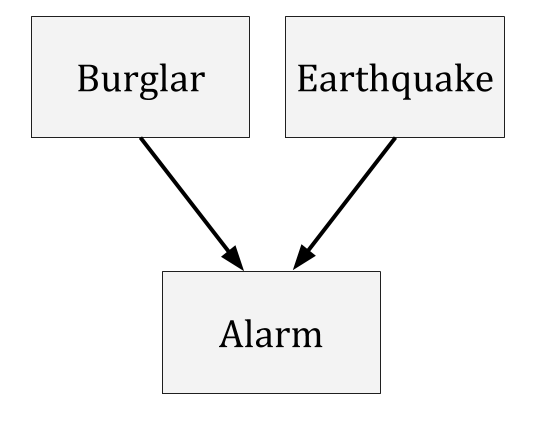
\includegraphics[width = 0.4\textwidth]{Assets/Explaining_Away.png}
\caption{The famous Burglar, Earthquake, Alarm network showing a minimal case of explaining away.}
\label{F:Explaining-Away}
\end{center}
\end{figure}
Knowledge of the state of the \texttt{alarm} makes \texttt{burglar} and \texttt{earthquake} dependent. The \texttt{alarm} is the observable variable here ($v$) and the \texttt{burglar} and \texttt{earthquake} are the hidden `causes` ($h$). For example if the \texttt{alarm} is true, and we see news of earthquake in the area, our belief that we have been burgled decreases. Expressed (again exemplify equation \ref{eq:sbn-factorisation}) in probabilities where $A$, $B$ and $E$ are the states of \texttt{alarm},\texttt{burglar} and \texttt{earthquake} respectively:
$$
P(A,B,E) = P(A|B,E)P(B)P(E)
$$

\subsection{Directed PGMs in Neural Networks: The Sigmoid Belief Network}

A Belief network can be expressed as a neural network, where conditional probabilities are parameterised as weights. \todowording{Simplify --- This network is called a Sigmoid Belief Network (SBN) as the probability of a variable $x_i$ being 1 that is dependent on a ancestor variable $parent_i$ the weighted sum into $x_i$, $\phi_i$ passed through the sigmoid function ($ \sigma(x)=1/(1+e^{-x})$)}. This is equivalent to a perceptron using a sigmoid activation function and ensures that the output is a valid probability (between 0 and 1).
SBNs take a naive approach to causes, where each hidden unit represent a single, simple cause. Formally, $\phi_i$ is a weighted sum of the activations of parent nodes:
$$ \phi_i = \sum_{j \in parent_i} W_{ij}x_j$$
and
$$
P(x_i = 1 | parent_i) = \sigma(\phi_i)
$$

\section{Undirected PGMs:}

Undirected PGMs do not represent causation, instead merely capturing a dependency between two units. These pairwise dependencies change the structure of the factorisation a factor $\Phi$ between each pair of variables $x_i,x_j$ resulting in the factorisation:
$$
P(X) = \frac{1}{Z} \prod_i \Phi(x_i, x_j)
$$
The introduction of the normalisation $Z$ (often referred to as the partition function) adds nontrival complexity to performing inference in Undirected PGMs~\todocite{}, a sum over all $2^N$ configuratiions of $x$ is required.

On the other hand, Undirected PGMs do not capture causal relationships. Calculating the state of a variable given another is no longer hampered by the effect of explaining away, however their reccurent structure, while expressive introduces an intractability in practice.

\subsection{Undirected PGMs in Neural Networks: The Boltzmann Machine}
A UPGM expressed as nueral network is referred as Boltzmann Machine or Markov Field, where connections encode dependancies with an associated weight. We see this where $W_{ij}$ is the weight between variables $x_i$ and $x_j$ the factor $\Phi$ is expressed as:
$$
\Phi(x_i, x_j) = e^{x_ix_jW_{ij}}
$$
The Boltzmann machine has proposed in various forms, from different domains throughout the years, for instance it was presented in a non-stochastic context of the Hopfield network in~\cite{Hopfield01041982}. Hinton and Sejnowski also proposed the Boltzmann machine in~\cite{geoffreye.hintonterrencej.sejnowski1983}. An example Boltzmann Machine is shown in figure \ref{F:Boltzmann-Machine}. As shown in this figure \ref{F:Boltzmann-Machine}, the Boltzmann Machine can be recurrent, expressing complex dependencies between variables. This recurrence makes inferring the state of a subset variables based on knowledge of another subset non-trivial as the size of the network grows\todocite{}.
\begin{figure}[h]
\begin{center}
  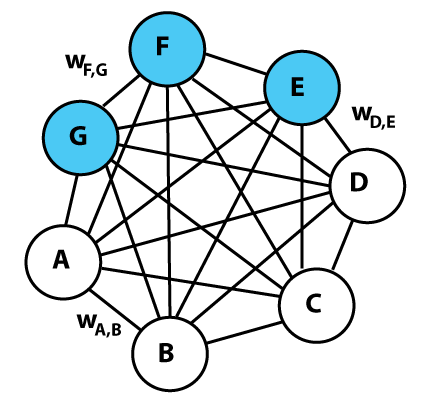
\includegraphics[width = 0.4\textwidth]{Assets/Boltzmann_Machine.png}
\caption{A Boltzmann Machine, the blue shaded nodes representing the observed variables, and the non-shaded nodes the latent variables.}
\label{F:Boltzmann-Machine}
\end{center}
\end{figure}

\subsection{Restricted Boltzmann Machines}


\todowording{A Boltzmann Machine's architecture can be altered to alleviate inference shortcoming. The restriction, originally proposed by \cite{Smolensky:1986vy}, and then later revitalised with a training algorithm that operates on the deeper architecture of the DBN~\cite{geoffreye.hintonterrencej.sejnowski1983}}. The restriction requires the network to be a two layer bipartite network, each layer corresponding to the observed (visible) and latent (hidden) units. Connections are forbidden between the layer of hidden units and the layer of visible units respectively. An example Restricted Boltzmann Machine architecture is shown in figure~\ref{F:Restricted-Boltzmann-Machine}. The collection of hidden units, forming a layer are referred to as the \texttt{hidden layer}. The collection of visible units are referred to as the \texttt{visible layer}.

\begin{figure}[h]
\begin{center}
  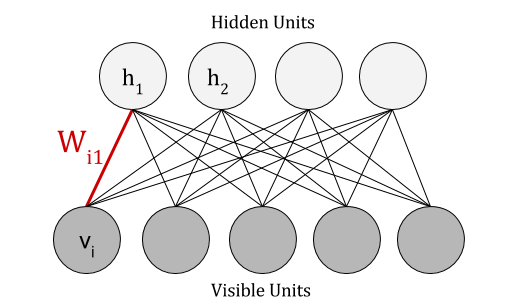
\includegraphics[width = 0.6\textwidth]{Assets/RBM_Example.png}
\caption{An example Restricted Boltzmann Machine with four hidden units, and five visible units. Note that the edges between units are not directed - representing a dependency not a cause. }
\label{F:Restricted-Boltzmann-Machine}
\end{center}
\end{figure}

% \subsection{Energy, and the log likelihood of the joint}
%
% An RBM models the joint distribution of hidden and visible states.
% The RBM assigns to every configuration of $h$ and $v$ an \texttt{Energy}, where the lower the energy, the more likely the RBMs configuration is to \textit{fall} into that state. Hopfield, in the context of what is now called the Boltzmann Machine~\cite{Hopfield01041982}, presented this energy as defined by the function as:
% $$ E(v,h) = -\sum_{i \in visible}{W_{0i}v_i}   -\sum_{j \in hidden}{W_{0j}h_j}  -\sum_{i,j}{v_ih_jW_{ji}}  $$
The probability of the RBM being in a given configuration is the joint probability of $h$ and $v$:
$$ P(h,v) = \frac{1}{Z} \prod_{j,i} e^{h_jv_iW_{ji}} $$
Taking logs this becomes:
$$ \log P(h,v) = \log \sum_{j,i} h_jv_i  W_{ji}  - \log Z $$
$ Z $ is the partition function, which normalises the probability of the joint. Calculating this would require summing over all $2^N$ configurations of $h$ and $v$, which is intractable for practical numbers of units. For instance a 28 by 28 image corresponds to 784 visible units, and for, say 10 hidden units this would amount to $ 2^{784} * 2^{10} $ possible configurations. We opt to work in terms of $P^\star$ which is the non-normalised probability of the joint over $h \text{ and } v$.
% So we arrive at:

\begin{equation}\label{eq:LogPJoint}
   \log P^\star(h, v) = \log \sum_{i,j} {h_j v_i W_{ji}}
\end{equation}

\section{Sampling in Generative Models}

\subsection{Why sampling is important}

Sampling is used when the distribution we want to work from is intractable to calculate analytically. As mentioned in \ref{S:Generative-Models}, the power of generative models is their ability to represent, reconstruct and be trained on data. These tasks all require sampling from configurations of the hidden and visible units, often conditioned one or the other. There are two cases:
\begin{itemize}
  \item Sampling from $P(v|h)$, which is known as running the generative model, where the model \emph{generates} data based on a hidden representation.
  \item Sampling from $P(h|v)$, which is known as \emph{inverting} a generative model (This is also refferred to as \emph{inference}). The process is called `Inverting` because instead of the model generating the data (sampling from $P(v|h)$) we instead try to infer a representation given data $P(h|v)$. It is the process of reasoning about what we do not know, given that of which we do.
\end{itemize}


Sampling from $P(v|h)$ and $P(h|v)$ is required to train generative models, as often the gradient to be climbed/descended involves calculating a probability over all the units in the generative model. Training a network based generative model involves calculating a weight update, which in turn requires inferring a hidden representation given a training item. The converse, sampling from a $P(v|h)$ is also required. \todocite{EM}

\todowording{inference for our purpose is used for (somehting about not training)}

\subsection{The sampling technique: Gibbs Sampling}

Gibbs sampling is a special case of Markov Chain Monte Carlo \cite{hastings70}, a technique for drawing sampling from a complex distribution. Sampling from the probability mass (or `joint distribution`) of a generative model is a common use case for Gibbs sampling~\cite{Pearl:1988:PRI:52121}.

Gibbs sampling explores the desired probability distribution, taking samples of that distribution's state, allowing iterations of exploration between drawing of a sample to ensure that the samples are independent\todocite{}. The process of taking a step between states is referred to as a \texttt{Gibbs iteration} or a \texttt{Gibbs Step}. Formally the algorithm is descibed in algorithm~\ref{Alg:Gibbs-Sampling}.

\begin{algorithm}[!ht]
 \KwData{A vector $x$ indexed by $j$.}
 \KwResult{Gibbs sampling algorithm}
 Let $ x_{\smallsetminus} j$ be all components that make up $x$ vector except $x_j$\;
 initialization, begin with $x$, we are going to get a sample $x'$\;
  \For{$k$ many iterations}{
   \For{each component in $x$, $x_j$}{
     Draw a sample, $x_j'$ from $P(x_j| x_{\smallsetminus} j)$\;
     Update the current value of $x_j$ in $x$ with $x_j'$\;
   }
  }
 \caption{The Gibbs Sampling Algorithm}\label{Alg:Gibbs-Sampling}
\end{algorithm}

\subsubsection{Mixing Time of the Gibbs Sampler}

MCMC methods aim to approximate a distribution, by exploring likely states. As we often start this process from a random state, it's important that enough Gibbs steps are taken before a sample is drawn. This is because the random state may not be close any part of the true distribution we want to sample from, so by running the chain for many iterations we increase the likelihood of samples being from the desired distribution.

This process of waiting for enough steps to before drawing samples is referred to as the \texttt{Mixing Time}. When Hinton when proposed a fast training for algorithm for RBMs and DBNs~\cite{Hinton:2006:FLA:1161603.1161605}, Gibbs sampling is used for performing inference in RBMs and as result also in the ORBM. The \texttt{mixing time}, that is how many Gibbs iterations are needed to reach a satisfactory sample is an important part issue in the ORBM, in that one Gibbs step was sufficient in practice for training and using an RBM. The new generative model is not so fortunate.



\subsection{Sampling in a Sigmoid Belief Network}


Sampling from $ P(v|h) $ (known as Ancestral Sampling) is extremely efficient in a SBN, it does not need Gibbs sampling. It can be expressed as
\begin{equation}\label{eq:SBN-v-given-h}
P(v|h) = \sum_i v_i \log \sigma_i(h) + (1-v_i)log(1-\sigma_i(h))
\end{equation}
As this process is calcuated by propagating probabilites from the root hidden causes, it is known in a SBN as Ancestral Sampling.

Conversly, sampling from $P(h|v)$ in an SBN is intractable. Performing inference in a Sigmoid Belief network would allow source separation, as each hidden unit could represent a simple cause. The SBN would be shown an input, and could extract representations of the seperate causes that likely gave rise to the input. There exist algorithms for performing inference in Sigmoid Belief Networks. For instance, the Belief Propagation algorithm proposed by Judea Pearl~\cite{Pearl1982} operates on this encoding, calculating the probabilities of a given network state (i.e. the state of all the variables). As well as constraining the architecture to be Directed Acyclic Graph, Belief Propagation is intractable to use as the number of variables grow\todocite{}. As we want to work with cases with upwards of 100 visible and hidden nodes, these algorithms break down.

Despite the Sigmoid Belief Network being expressive and providing a succinct encoding of conditional probabilities, Gibbs sampling is intractable for SBNs of practical size~\cite{Jensen95blockinggibbs}. The issue being that the Gibbs chain takes too long to mix~\cite{neal1992:connectionist}, which arises from the the `explaining away effect`~\cite{Hinton:2006:FLA:1161603.1161605}. Calling back to the example in section \ref{}, instead of a single \texttt{burglar} or \texttt{earthquake} becoming dependant given the \texttt{alarm}, there is more in the realm of hundreds of burlgars and earthquakes all suddenly depedendant.

Being able to efficiently sample from $P(h|v)$ is also required for training generative models\todocite{em} making Sigmoid Belief Networks impractical for not only inference, but also training.




\subsection{Gibbs Sampling in a Boltzmann Machine}

Performing Gibbs sampling appears trivial in a Boltzmann Machine, in that to find the probability of a given unit being active a weighted input to that node is passed through a sigmoid function. However, in practice the recurrent nature of Boltzmann Machines makes sampling intractable as updating a node will change the probabilities of those connected. However, it was shown that given unlimited training time Boltzmann Machines could be trained, out performing the state of the art models of the time \todocite{This}.

Recall that $ x_{\smallsetminus} j$ be all components that make up $x$ vector except $x_j$ and that a Boltzmann Machine has symmetric weights ($ W_{ji} = W_{ij} $),
$$
P(x_j = 1, x_{\smallsetminus}j) = \frac{1}{1 + e^{-\sum_i w_{ji}x_i}}
$$
That is, Gibbs sampling in a Boltzmann Machine amounts to use the Sigmoid function of the weighted inputs.
\todocite{neal1992:connectionist}

\subsection{Gibbs Sampling in RBMs}

A big payoff for the restriction in an RBM is inverting the model becomes tractable, as the latent variables no longer become dependant given the observed variables. This is illustrated in figure~\ref{F:Restricted-Boltzmann-Machine} the hidden unit $h_1$ is not dependent on $h_2$ wether or not we know anything about the visible units. Firstly, this is the opposite of a SBN, where knowledge of the visible units makes the hidden units dependant. Secondly, by removing the recurence present in Boltzmann Machines, it reduces the expresiveness of the RBM network while making the RBM useable in practice as the Gibbs sampling process can stop after one Gibbs step\todocite{}.

In order to describe Gibbs sampling in the new architecture proposed, it must first be explained for a standard RBM --- The process of Gibbs sampling is as follows:
  \begin{itemize}
    \item One must sample from $P(h|v)$ giving a hidden state $\tilde{h'}$
    \item Using this hidden state, a visible state is then generated, $\tilde{v'}$, by sampling from $P(\tilde{v'}|\tilde{h'})$. This process of generating a hidden pattern, and subsequent visible pattern is referred to as a Gibbs step.
    \item This chain of Gibbs steps between sampling from $P(h|v)$ and $P(v|h)$ can then be repeated as desired, the longer the chain the closer the samples will be to the true joint distribution that the model has learnt. For training an RBM Hinton\todocite{CD-1Paper} showed that 1 step is often enough in practice, as one step is enough to infer a direction to adjust the weights in.
  \end{itemize}
  The process of updating the hidden, then visible layers forms what is referred to as the \texttt{Gibbs Chain} and is visualised at layer level in figure \ref{F:Gibbs_Chain}.
  \begin{figure}[h]
    \begin{center}
      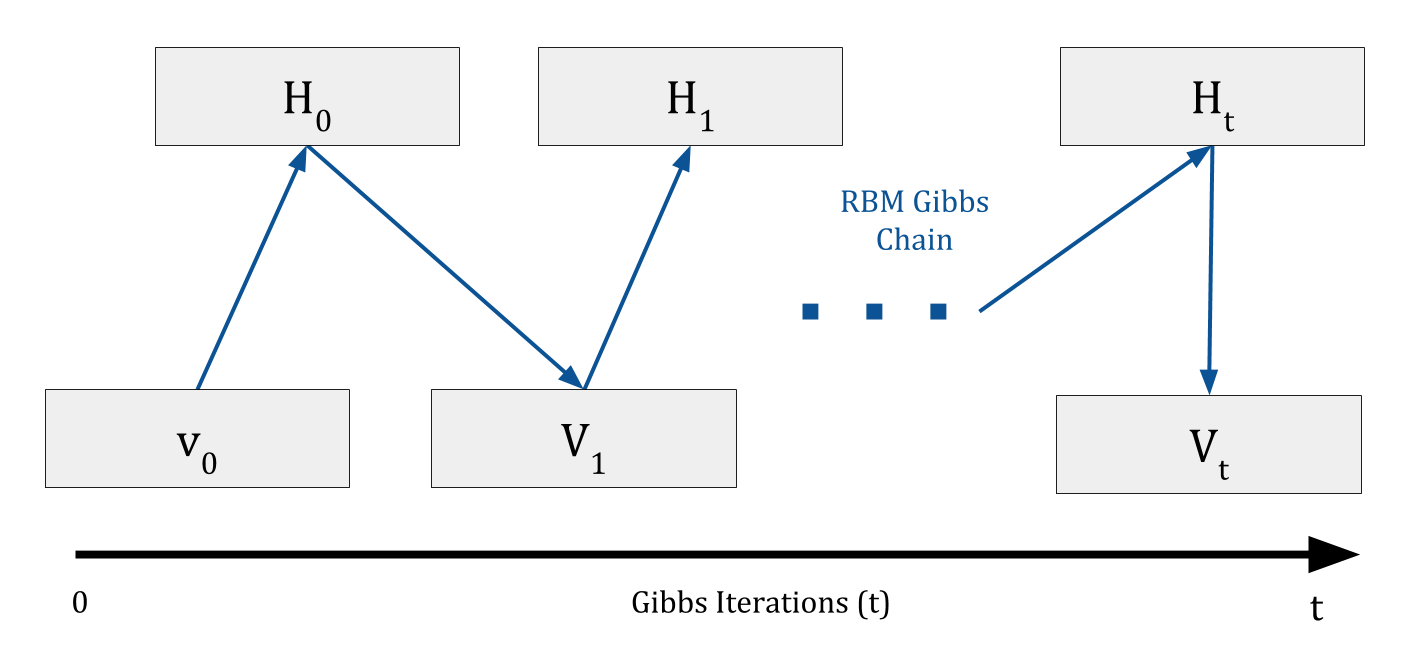
\includegraphics[width=0.8\textwidth]{Assets/RBM-Gibbs-Chain.png}
    \end{center}
    \caption{A figure illustrating a Gibbs chain where left to right indicates a Gibbs iteration. Note this is \emph{not} a PGM.}
    \label{F:Gibbs_Chain}
  \end{figure}

  \subsubsection{The Gibbs update}\label{S:Gibbs-Update}

    Denote the Gibbs sampler's probability of setting a variable, $x_j$ to 1 as:
    \begin{equation}\label{eq-p1-gibbs-full}
    P_{Gibbs}(h_j = 1 | v, h_{k != j})
    \end{equation}
    We can refer to the proability in equation \ref{eq-p1-gibbs-full} as $p_1$ and the converse $P_{Gibbs}(h_j = 0 | v, h_{k != j})$ can be referred to as $p_0$.
    Then, by the product rule of probabilities:
    $$
    \begin{aligned}
    \frac{p_1}{p_0} &= \frac{P^\star(h,v \text{ where } h_j = 1)}{P^\star(h,v \text{ where } h_j = 0)}\\
    &= \frac{p_1}{1 - p_1} \\
    % \text{Rearranging to give p_1 leads to} \\
    p_1 &= \frac{1}{1 + \frac{P^\star(h,v \text{ where } h_j = 0)}{P^\star(h,v \text{ where } h_j = 1)} }
    &= \frac{1}{1 + e^{-\psi_j}}
  \end{aligned}
    $$
  To update a hidden unit $h_j$
  we find $ P(h_j = 1 | v) $ where $v$ is an input pattern. In the context of an image, $ v $ would be the pixel values where each pixel corresponds to a visible unit, $v_i$.
  The probability of a given hidden unit activating is: \todocite{Gibbs sampling would be good here}.
    \begin{equation}\label{eq:Hid-Gibbs-Update}
    P(h_j = 1 | v) = \sigma(\psi_j)
    \end{equation}
    Where $\psi_j$ is the weighted sum into the $jth$ hidden unit and $\sigma()$ is the Sigmoid function, or it also known as the Logistic function $\sigma(x)=1/(1+e^{-x})$. Figure \ref{F:PSI} illustrates $\psi_j$ for an example RBM.
    \begin{figure}[h]
    \begin{center}
      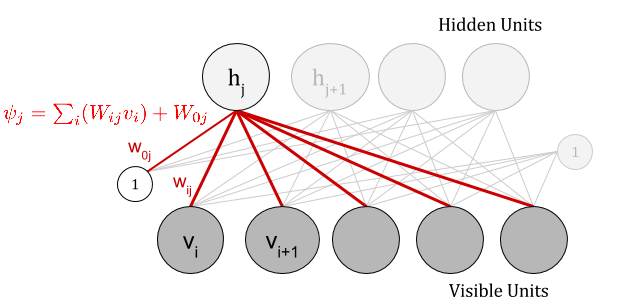
\includegraphics[width = 0.8\textwidth]{Assets/PSI_and_PHI.png}
    \caption{A diagram showing $\psi_j$, the weighted sum into the $jth$ hidden unit. Note that $W_{oj}$ is the hidden bias, represented as a unit that is always on with a weight into each hidden unit.}
    \label{F:PSI}
    \end{center}
    \end{figure}
    As the weights are symmetric, sampling from the visible layer, given a hidden state is similar. That is $P(v_i = 1 | h)$, where $h$ is the entire hidden vector is given by:
    \begin{equation}\label{eq:Vis-Gibbs-Update}
     P(v_i = 1 | h) = \sigma(\phi_{i})
    \end{equation}
    Where $\phi_i$ is the weighted sum into the $ith$ visible unit, which is: $ \phi_i = \sum(W_{ji}h_{j}) + W_{0i} $. Both $\phi_j$ and $\psi_i$ can be expressed in alternative, but useful way:
    \begin{equation}
    \phi_j = \log P^\star(v,h | v_i = 1) - \log P^\star(v,h | v_i = 0)
    \end{equation}
    \begin{equation}\label{psi-gibbs-update-rbm}
    \psi_i = \log P^\star(h,v | h_j = 1) - \log P^\star(h,v | h_j = 0)
    \end{equation}



\subsubsection{Reconstructions: visualising what the RBM has learnt}

RBMs create an internal representation given an input by sampling from $P(h|v)$. They can also generate a faux input given an internal representation. Performing one Gibbs iteration, that is, sampling from the hidden units given a `clamped` input $ P(h|v) $ and then taking the generated hidden state and generating a faux input (sampling from $P(v|h_{sampled})$) results in a \texttt{reconstruction}. Clamped input is where the visible units are set to be an input pattern. The model tries to reconstruct the input based on the internal representation it has learnt to model. This has applications in increasing the size of a dataset by introducing variation by generatin these faux inputs\todocite{}.

\subsubsection{RBM Fanstasies: The Free-Phase of a Generative model}

In the same way that a Generative model uses reconstructions to try and recreate the supplied input vector, performing many, many (greater than 100) Gibbs iterations with no input pattern clamped allows the reconstructions to explore the probability mass that has been built by the model during training. Sampling from these wanderings creates what are refferred to as `fantasies` or `dreams`. These give a sense of what the model has learnt, and can act a smoke test for if the model has actually capture anything.
\todocite{(TODO-CITE-PAPER-WITH-MNIST-DREAM-EVALUATION, they were crappy)}.

%
% \subsection{Terminology in Generative Models observable and hidden variables}
%
% Connections between units are used to encode relationships between the variables, where the relationship may be causal, such as in a Sigmoid Belief network or an encoding/representation in the Restricted Boltzmann Machine.
%

% \subsection{PGMs as a tool reasoning about generative models}
%
% Probalistic Graphical Models or PGMs for short, are an expressive way to represent a collection of related, stochastic variables. If the graph is directed then the edges represent causation, this is also referred to a Bayesian network. Conversely, if the graph was undirected then edges represent a dependancy or mapping.

%   \section{An intractable model for causes}
%     \subsection{Sigmoid Belief Networks}
%
%     The ORBM relies on the Sigmoid Belief Network to capture the causation. The Sigmoid Belief Network (SBN) is composed of units with weights and a sigmoid activation function, akin to that of a perceptron linear threshold unit/Perceptron. The probability of a node being `on` is found by taking the weighted sum of all input to that node and applying a Sigmoid function or another activation function that ensures a values between $0$ and $1$.
%
%     SBNs offer a way to model causation in machine learning, as every hidden unit represent a single, simple cause. Nodes in the network represent binary variables which are dependent on ancestor nodes, the degree of which is encoded in a weight on a directed edge between them.
%
%
%
%     \subsection{Explaining Away --- a trade off between modeling causes and tractability}\label{SS:Explaining-Away}
%
%     The benefit of the Belief Network is also it's weakness, a structure that models a system of interest inherently has dependancies. In its minimal case explaining away can be seen in a 3 node network popularised by David Barber in his book \cite{Barber:2012:BRM:2207809}, as shown in figure \ref{F:Explaining-Away}. Each of the nodes represents a binary state. For instance $Burglar = 1$ means that the person owning the \texttt{Alarm} has been burgled. Also note how the connections between the units have arrows, this conveys causation.
%
%
%     In the network shown in figure \ref{F:Explaining-Away}, knowledge of the \texttt{Alarm} creates a dependance between \texttt{Burglar} and \texttt{Earthqaukes}. For instance, say the Alarm has gone off and we know an earthquake has occurred, our belief in being burgled decreases. The dependance in belief networks means that sampling from the network requires a longer Markov Chain to mix, as changing the value of \texttt{Earthquake}, effects the value of \texttt{Burglar}. In a network with many connected nodes the dependence introduced makes sampling take longer. In the context of images, where there may be upwards of 1000 observable values, all with different dependancies this becomes intractable. Neal showed this by comparing the number of gibbs iterations required for small enough error rates in~\cite{neal1992:connectionist}.
%
%   \subsection{Boltzmann Machines}
%
% A Boltzmann machine has proposed in various forms throughout the years from different backgrounds, for instance Paul Smolensky presented it in context of  `Harmony Theory` \cite{Smolensky:1986vy}. Where-as Hinton and Sejnowski also propsed the Boltzmann machine in~\cite{geoffreye.hintonterrencej.sejnowski1983}. The Boltzmann Machine has qualities in common with Belief Networks. Both are generative models with their nodes having probabilities of being active based on neighboring nodes. Connections between nodes have associated weights as shown in figure \ref{F:Boltzmann-Machine}. These weights are symmetric.
% Unlike a Belief Network, a Boltzmann Machine is a undirected network that allows cycles and thus more complex relationships can be captured. Also connections no longer encoe causal information, instead they encode a dependency.
%
%
%   \section{Restricted Boltzmann Machines: A Strong assumption}
%
%   While Boltzmann Machines are impractical to train and sample from as networks grow in size \todocite{} their architecture can be altered to alieviate these shortcomings. The restriction, originally proposed by \todocite{Hinton, a proper cite}, and then later revitalised with a deeper architecture training algorithm in Hintons \cite{geoffreye.hintonterrencej.sejnowski1983}. The restriction requires the network to be a two layer bipartite network, each layer corresponding to the observed (visible) and latent (hidden) units. Connections are forbidden between the layer of hidden units and the layer of visible units respectively. An example Restricted Boltzmann Machine architecture is shown in figure~\ref{F:Restricted-Boltzmann-Machine}. The collection of hidden units, forming a layer are referred to as the \texttt{hidden layer}. The collection of visible units are referred to as the \texttt{visible layer}.
%

%   \subsection{Gibbs Sampling in RBMs}
%
%   In order to describe Gibbs sampling in the ORBM, it must be first introduced in the context of RBMs. For the following discussion, the hidden units are indexed by $j$ and the visible units are indexed by $i$.
%   To perform inference, create reconstructions, and train RBMs, Gibbs sampling is used to draw samples from $P(h|v)$ (referred to as sampling from the posterior) and $P(v|h)$ respectively. It is introduced here to be reference later in Gibbs in an ORBM. In an RBM the process of Gibbs sampling is as follows:
%   \begin{itemize}
%     \item One must sample from $P(h|v)$ giving a hidden state $\tilde{h'}$
%     \item Using this hidden state, a visible state is then generated, $\tilde{v'}$, by sampling from $P(\tilde{v'}|\tilde{h'})$. This process of generating a hidden pattern, and subsequent visible pattern is referred to as a Gibbs step.
%     \item This chain of Gibbs steps between sampling from $P(h|v)$ and $P(v|h)$ can then be repeated as desired, the longer the chain the closer the samples will be to the true joint distribution that the model has learnt. For training an RBM Hinton showed that 1 step is often enough in practice, as one step is enough to infer a direction to adjust the weights in.
%   \end{itemize}
%    This process can be calculated in one step for all units in the target layer as they are independant of one another. The process of updating the hidden, then visible layers forms what is referred to as the \texttt{Gibbs Chain}. \todocite{Feel like I could  cite this again in like a CD paper or something.} This process is visualised at a layer level in figure \ref{F:Gibbs_Chain}
%
%   \begin{figure}[h]
%     \begin{center}
%       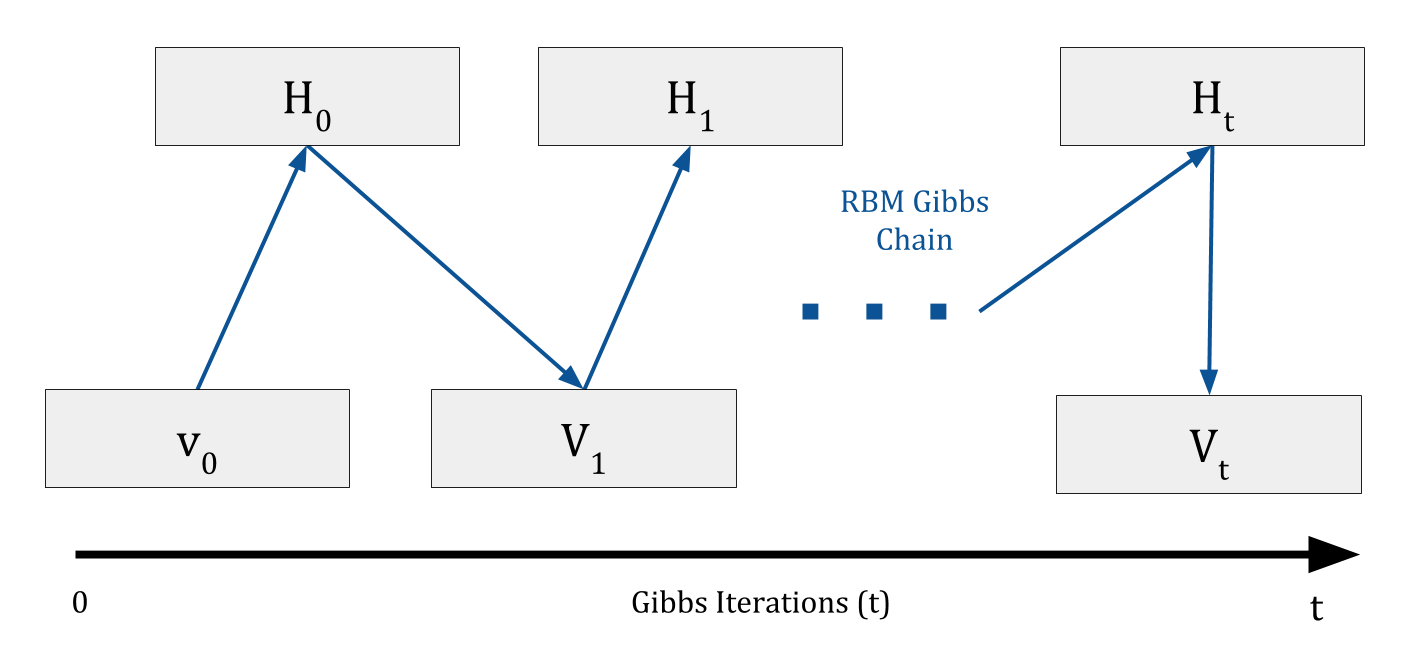
\includegraphics[width=0.8\textwidth]{Assets/RBM-Gibbs-Chain.png}
%     \end{center}
%     \caption{A figure illustrating a Gibbs chain where left to right indicates a Gibbs iteration. Note this is \emph{not} a PGM.}
%     \label{F:Gibbs_Chain}
%   \end{figure}
%
%   \subsubsection{The Gibbs update}\label{S:Gibbs-Update}
%
%   In a standard RBM, updating a hidden unit $h_j$ when performing Gibbs sampling is calculated by finding $ P(h_j = 1 | v) $ where $v$ is an input pattern. In the context of an image, $ v $ would be the pixel values where each pixel corresponds to a visible unit, $v_i$.
%   The probability of a given hidden unit activating is: \todocite{Gibbs sampling would be good here}.
%   \begin{equation}\label{eq:Hid-Gibbs-Update}
%   P(h_j = 1 | v) = \sigma(\psi_j)
%   \end{equation}
%   Where $\psi_j$ is the weighted sum into the $jth$ hidden unit and $\sigma()$ is the Sigmoid function, or it also known as the Logistic function $\sigma(x)=1/(1+e^{-x})$. Figure \ref{F:PSI} illustrates $\psi_j$ for an example RBM.
%
%   \begin{figure}[h]
%   \begin{center}
%     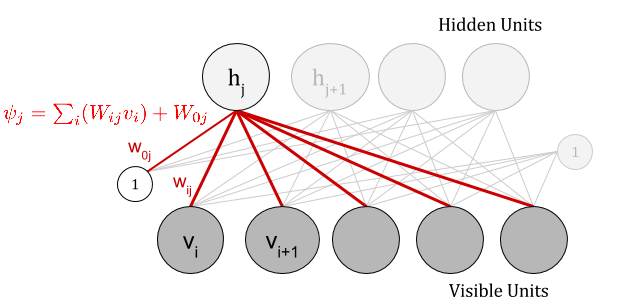
\includegraphics[width = 0.8\textwidth]{Assets/PSI_and_PHI.png}
%   \caption{A diagram showing $\psi_j$, the weighted sum into the $jth$ hidden unit. Note that $W_{oj}$ is the hidden bias, represented as a unit that is always on with a weight into each hidden unit.}
%   \label{F:PSI}
%   \end{center}
%   \end{figure}
%
%
%
%   As the weights are symmetric, sampling from the visible layer, given a hidden state is similar. That is $P(v_i = 1 | h)$, where $h$ is the entire hidden vector is given by:
%   \begin{equation}\label{eq:Vis-Gibbs-Update}
%    P(v_i = 1 | h) = \sigma(\phi_{i})
%   \end{equation}
%   Where $\phi_i$ is the weighted sum into the $ith$ visible unit, which is: $ \phi_i = \sum(W_{ji}h_{j}) + W_{0i} $. Both $\phi_j$ and $\psi_i$ can be expressed in alternative, but useful way:
%   \begin{equation}
%   \phi_j = \log P^\star(v,h | v_i = 1) - \log P^\star(v,h | v_i = 0)
%   \end{equation}
%   \begin{equation}\label{psi-gibbs-update-rbm}
%   \psi_i = \log P^\star(h,v | h_j = 1) - \log P^\star(h,v | h_j = 0)
%   \end{equation}
%
%
%
%
%     % \subsubsection{Tractable Training - Contrastive Divergence}
%     % Hinton TODO-CITE-CLASSIC-PAPER proposed Contrastive Divergence as a method for training RBMs efficiently. The algorithm leverages the now tractable wake phase because $P(h|v)$ is efficeint to compute. However the free or sleep phase required another restriction where the network is only left to its own dynamics can be limited to only one iteration and still perform well. TODO-CITE-CD-PAPER
%
%     % This restriction allows an efficient calculation of the Wake Phase of generative model learning, as the $ P(h|v) $ can be calculated as a simple weighted sum passed through a sigmoid followed by a bernouli trial where the probability of being $1$ is equal to the result of sigmoid.
%
%
%
%   % \subsection{Deep Learning}
%   %
%   %   \begin{itemize}
%   %     \item Discuss deep learning as there are clear parallels to Deep Belief Networks and the new approach
%   %     \item in paritcular how the deep networks have this process of freezing the weights and creating a sigmoid belief layer instead. There seem to be clear parallels between a deep network with one RBM to the ORBM.
%   %   \end{itemize}
%   %
%   % \begin{itemize}
%   %   \item Unrolling the gibbs chain and we are in effect training an infinite depth sigmoid beleif net (TODO-REFERENCE-HINTONS-PAPER-HERE)
%   % \end{itemize}
%

%
% \chapter{Design and Implementation}\label{C:work}

A significant hurdle for the project was gaining enough understanding of the existing work on RBMs to be able to implement the ORBMs algorithm and architecture. This was crucial as an incorrect implementation invalidates  contributions \ref{item-c2} and \ref{item-c3} of this project.


\section{Implementation Design}

\begin{itemize}
  \item Ordering of evaluation tasks made unit testing, with hand made test cases possible. Also less risk, remove the uncertainty around the RBM.
  \item testing approach
\end{itemize}

\subsection{Language Choice}

\todowording{The implementation of the ORBM and inference algorithm is in \emph{Python}, with \emph{Matlab} and \emph{Java} being the other languages considered.}

I have spent my University career working in Java, and nowdays it is efficient to perform machine learning tasks. Python's module and class system promotes composition, and multiple inherietance in particular allows for composition of different classes.

Matlab is a popular numerical computing environment\todocite{} and has a lot of online resources as well as machine learing papers \todocite{} that include snippets or full Matlab programs that were used in the paper. Also Matlab is built around strong, efficient support for matrix operations which are very prolific in the RBM and ORBM implementations and evaluations.

Python has a very sucinct syntax and shallow learning curve\todocite{}, as well as being the langauge of choice of my supervisor. \todowording{This is favourable as I can have support for translating the algorithm into python correctly.} Through libraries that supply wrappers for C-bindings, efficient code can be written but overal being an interpreted language Python is slower than Matlab and Java\todocite{}. Three main factors influenced the choice for python:

\begin{description}
\item[Up front learning] Given the amount of up front learning of concepts required to implement the solution, Python was favoured over Java or Matlab because is has a very shallow learning curve. Despite having expeirence in Java as well as Python, I had never used machine learning or linear algerbra libraries in either languages. Given the amount of up front learning required to understand the concepts in this project let alone implement it, I opted for the shallower learning curve of Python. Also my supervisor has experience using Python and the libraries involved with this project. A shallower learning curve meant that more time could be allocated to the evaluation which is the foremost contribution of this project.
\item[Library Support] Matlab and Python were two contendors in this factor, as a lot of matlab machine learning code is avaliable with supporting papers \todocite{}. Python has libraries such as NumPy, SciPy and Matplotlib \todocite{} which mirror Matlabs functionality. However, NumPy and SciPy are all open source, while there is argument for treating an API as a black box --- i.e. not writing code that is dependant on the underlying implementation, having the option to view source helped me better grasp the concepts. In particular being able to compare my implementation of the RBM to Sklearn's \todocite{} allowed for some performance improvements.
\item[Ease of Evaluation] Python provides strong plotting library that is inspired by Matlab and R --- MatplotLib \todocite{}. Matplotlib is interoperable with the NumPy library, meaning that turning results into plots was really easy.

Also the evalation requires repeateldy running a test to gain more confidence in the stochastic result. This is made possible by the ECS-Grid \todocite{}. Python is supported with very minimal extra work required. A simple script that manages input and output is required. However the Java support on the ECS grid requires significantly more setup \todocite{}. \todowording{This seemed like an unnesccariy risk to introduce to the project at the later stage in the project where evaluation is being carried out.}
\end{description}
%
% All of the languages considered have the efficiency for machine learning tasks, despite Python being on the slower end of the spectrum of languages, versus that of the compiled JVM languages like Matlab or Java, it is still fast enough. The complexity of the traditional RBM is relative to what is trying to be modelled, less of the language implementing it.
% Java and Python have robust testing suites given they are used for non-academic goals. Matlab and R do have suites however the author has not had experience with them. Choosing from one of these two languages would increase the amount of upfront learning required and therefore increase this risk.
% The author had the most experience with Python and Java, however Python was favoured due to it's Matlab-like library NumPy. Expressive matrix syntax combined with the familiarity and brevity of Python made it a compelling option.


\subsection{Program Architecture}

The implementation of the RBM, ORBM and algorithm is implemented with unit testing and composability in mind. It is important that the design supports comparing the Full and Approximated Correction\todocite{Equation ..}. By using Python, multiple inheritance could be leveraged to achieve this composability. For instance  adding continuous pixel value support to the \texttt{Full Correction Sampler}, one simply needed to extend \texttt{Continuous Approximate Correction Sampler} and the  \texttt{Full Correction Sampler}, with no code actually in the new class. The architecture is pictured in the class diagram \ref{F:Prog-Arch}. There were three main roles these classes filled:
\begin{enumerate}
  \item The \texttt{Trainer} was used to train the weights of a supplied \texttt{RBM}. It would do so using a supplied \texttt{sampler}, decoupling how samples were generated from the training process.
  \item The \texttt{RBM} was the model of an RBM, storing the weight matrix, as well as parameter information. Also this supported conversion of the SciPy Sklearn libraries' RBM implementation into the implementation used in this project. Decoupling the concept of an \texttt{RBM} from the \texttt{Sampler} and the \texttt{Trainer} meant that RBMs could be `plugged` into the ORBM architecture with ease.
  \item The \texttt{Sampler} defined how to perform Gibbs sampling, the subclasses defining whether it is standard RBM sampling or ORBM sampling. This made is trivial to compose samplers, which was required for the ORBM samplers.
\end{enumerate}

\begin{figure}[h]
\begin{center}
  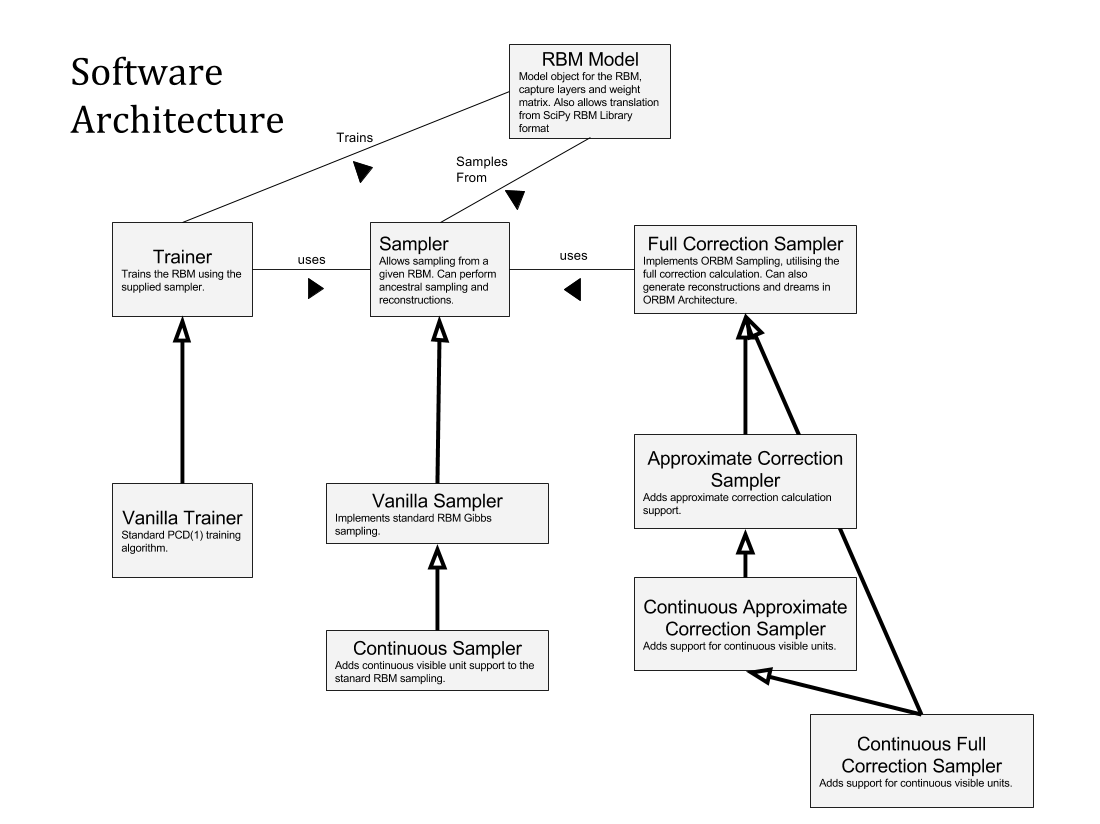
\includegraphics[width = 1\textwidth]{Assets/ENGR489-Architecture.png}
\caption{A figure showing the architecture for the implemented test suite in UML notation.}
\label{F:Prog-Arch}
\end{center}
\end{figure}

\subsection{Testing Approach}

The inference algorithm is the most crutial part of the implementation to test. In larger dimentional tasks, unit testing to ensure the algoruhtm produces the correct values becomes difficult. In smaller cases I was able to ensure the probabilities of $P(h|v)$ and $P(v|h)$ calculated by the implementation matches calculations I made by hand. Being an unsupervised black boxes, determining if an RBM (and by extension the ORBM) hidden representation is `correct` for larger tasks such as the MNIST handwritten digit dataset is non-trivial. Concerned by this risk, I designed my evaluations to build confidence in the algorithm and the implementation.

\section{Evaluation Design}

\subsection{Examining the mixing time of inference in the ORBM}

As described in Section \todocite{\ref{}}, sampling from $h^A$ and $h^B$ suffers from the effect of explaining away (\todocite{\ref{}}) which requires a Gibbs chain to run. While intractable for a large SBN, as only two causes are being modelled, ideally the Gibbs chain for this process won't take many iterations to mix. As the correction needs to be computed for each Gibbs iteration, a long Gibbs chain could be detrimental to performance.
Finding this \emph{optimal mixing time} for the ORBM is only an issue as the number of dimensions and training examples increase. In smaller dimensions mixing can be overcome by using a large ($>1000$) number of Gibbs iterations. However in the larger problems this becomes intractable, so an optimal mixing time is desired.

This project examines the mixing time by way of examining reconstructions at various points of the Gibbs chain. This is also interesting in that we can observe the dynamics of the network and the effect of apply the \emph{correction} has on reconstructions. \todocite{Hinton has shown this in practice as a useful thing to observe, cite his movies.}.

\subsection{Evaluating RBMs and ORBMs}

  A challenge faced by this project and work with RBMs is that they are non-trivial to evaluate \todocite{}. Being unsupervised black box, one cannot merely inspect the hidden units for an input and be sure that a good model has been learnt. As I plug RBMs into the ORBM architecture it is important for the overal results that the RBMs are well trained.

\subsection{Hinton diagrams}
  We can examine the weights into a given hidden unit in the shape of the visible vector. For instance in the context of images, \texttt{Hinton Diagrams} allow visualisation of what a given hidden unit is `doing` by visualising the matrix. This was first used by Hinton in the context of Boltzmann Machines in \cite{Hinton:1986:LRB:104279.104291}. They also give insight into hidden unit utilisation. Weights are often initialised to small random values resulting in a Hinton diagram with little structure to it. This is illustrated in figures \ref{F:Hinton-Good} and \ref{F:Hinton-Bad}. The former showing a hidden units weights where some structure has been learnt, and the latter showing the opposite.

  \begin{figure}[htb]
  \centering
  \begin{subfigure}[t]{0.3\textwidth}
      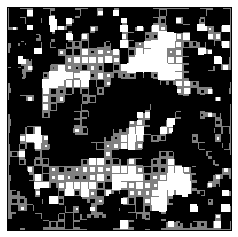
\includegraphics[width=\textwidth]{Assets/HINTON1.png}
      \caption{Utilised hidden unit Hinton Diagram}
      \label{F:Hinton-Good}
  \end{subfigure}
  ~ %add desired spacing between images, e. g. ~, \quad, \qquad, \hfill etc.
    %(or a blank line to force the subfigure onto a new line)
  \begin{subfigure}[t]{0.3\textwidth}
      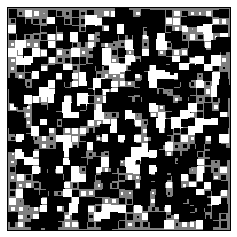
\includegraphics[width=\textwidth]{Assets/HINTON2.png}
      \caption{Unutilised hidden unit Hinton Diagram}
      \label{F:Hinton-Bad}
  \end{subfigure}
  \caption{Hinton Diagrams illustrating a trained hidden unit, versus that of an untrained/unutilised hidden unit. This is with no measures to enforce sparsity.}\label{fig:mnist-worse-best-results}
\end{figure}

\subsection{Reconstructions: a measure of performance}

Reconstructions, as described in Section \ref{SS:RBM-Reconstructions}, are a good measure of performance. \todocite{Hinton showed this in papers, also cite more ppapers showing reconstruction use. starting from early RBM training papers by Hinton, up to more recent in deeper networks - the goal being to show the reader that reconstructions are used well in practice.} Given the precident for using reconstructions as a performance measure, they will be the main way I evaluate the RBM in comparison to the ORBM. To be able to use this reconstruction based evaluation, knowledge of the ground truth was required. This was so:
\begin{itemize}
  \item RBMs could be trained and then plugged into the ORBM network.
  \item Reconstructions could be compared directly (by score) to the ground truth.
\end{itemize}



\subsection{Evaluating RBMs: Problem dependent}

  Evaluating RBMs is problem dependant, we can examine the different approaches avaliable by splitting problems into two cases:
  \begin{description}
  \item[Problems with small dimentionality] When the dimentionality of the input is very small ($<10$) and all possible inputs are known we can perform analytical evaluations of the RBM. By clamping the visible units of the RBM to each input in the training set, reconstructions can be created. This process can be repeated for each input, recording the frequency that each reconstruction occurs on a bar graph. We can then ensure that the RBM is reconstructing the input perfectly. For instance, an RBM trained on two bit XOR and clamped to the input $[1,0]$, might have a bar graph of reconstructions as illustrated in figure \todocite{\ref{F:Two-Bit-RBM-Recons}}.

  In a similar way to the reconstructions, samples can be drawn from RBM in a `free phase` without the input clamped to a given visible. The bar graph should exhibit dream visible patterns from the whole training set approximately an equal amount. Using the two bit XOR example once more, an example bar graph is shown in figure\todocite{\ref{F:XOR-ORBM}}.


  \begin{figure}[htb]
  \centering
  \begin{subfigure}[t]{0.4\textwidth}
      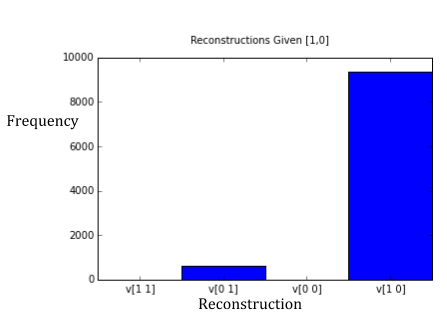
\includegraphics[width=\textwidth]{Assets/Two-Bit-RBM-Recon.png}
      \caption{Example reconstructions for the Handcrafted RBM, For 10000 independant reconstructions given the input $[1,0]$.}
      \label{F:Two-Bit-RBM-Recons}
  \end{subfigure}
  ~ %add desired spacing between images, e. g. ~, \quad, \qquad, \hfill etc.
    %(or a blank line to force the subfigure onto a new line)
  \begin{subfigure}[t]{0.4\textwidth}
      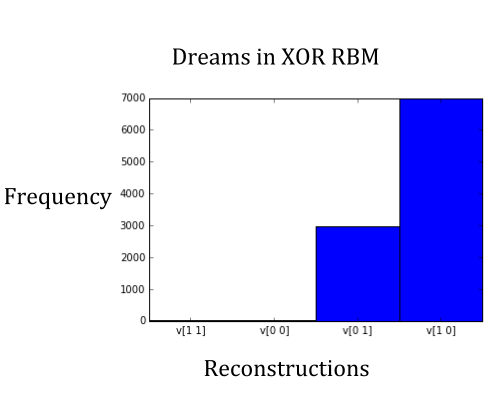
\includegraphics[width=\textwidth]{Assets/XOR-RBM-Dreams.png}
      \caption{Dreams in the XOR RBM, note how only the training data is present.}
      \label{F:Two-Bit-RBM-Dreams}
  \end{subfigure}
  \caption{Bar graphs exmplifying the use of reconstructions and dreams for small numbers of RBMs.}\label{F:XOR-Example-Plots}
\end{figure}


  \item[Problems  with large dimentionalities] In non-trivial cases, with larger datasets, reconstructions can be inspected and compared to the training dataset. However, empirically detecting if a model is trained is difficult, especially given the unsupervised, black box nature of RBMs.
  Alternatively, a `score` can be assigned to each item in the training set based on how well the RBM can reconstruct it. However in large cases your training set will not be complete --- you will not have every possible valid image like you would in a case where your images are 2 pixels.
  Dreams can also be examined in larger cases, but emperically detecting if they are `correct` is infeasible. Nevertheless, Dreams are useful to examine as dreams that look like items in the training set gives confidence the RBM \todowording{has learnt something.}

\end{description}


\todowording{My \todowording{x experiements} all followed the same high level process, working from trivial cases to more challenging tasks. The reason for this being that trivial cases make unit testing feasible, therefore ensuring conclusions can be drawn with regard to the algorithm and model, not an incorrect implementation.} By incrementally increasing the difficulty of the task, it allows me to identify what qualities of the problem make the algorithm less or more effective.

The evaluations in this project aimed to evaluate the ORBM and it's inference algorithm by examining reconstructions given a \todowording{multi-subject image}. Because the multi-cause inputs were images composed of known images, I could then compare the reconstructions to the ground truth. An example of a multi-cause input with two quadrilaterals is shown in figure \ref{F:Composite-Example}. The optimal reconstructions are equivalent to the two images that combined form the input.

\begin{wrapfigure}{r}{0.6\textwidth}
  \begin{center}
    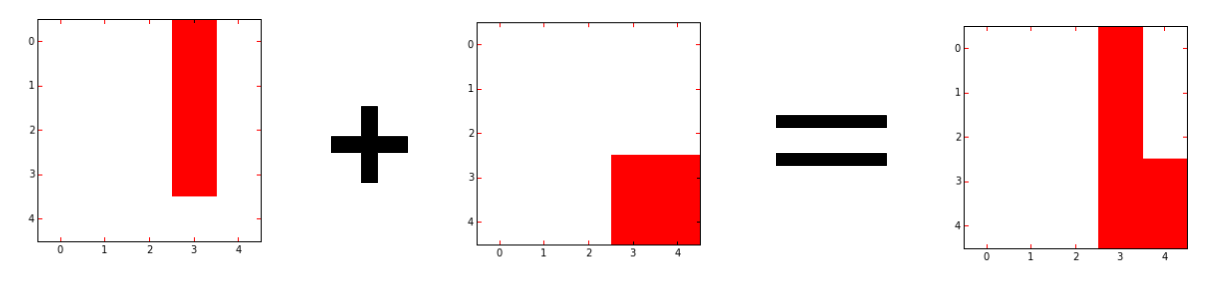
\includegraphics[width=0.48\textwidth]{Assets/Composite-Example.png}
  \end{center}
  \caption{A figure illustrating two five by five pixel images combining to form a composite/multicause input. The images are binary.}
  \label{F:Composite-Example}
\end{wrapfigure}

In the smaller dimenisonal cases the reconstructions are inspected by plotting the reconstructions and the frequency with which they occurred after a large amount of repetitions. In the larger dimensional tasks, two `scores` are used to evaluate reconstructions against the corresponding item of the training set.



\subsection{Choice of Evaluation Datasets}

As my evaluations follow the same outline of training RBMs, pluging them into the ORBM, and evaluating the reconstructions, the aspect of the evaluation that needs to be designed is the datasets for these tasks. It is important the images of the datasets are \emph{multi-subject} and that the individual images used to compose the training images are known. This is to allow the reconstructions of the ORBM (and RBM) can be compared to these underlying images, exploring how well the ORBM and RBM can perform source separations.

\begin{itemize}
  \item 2 Bit XOR --- The minimal case of image source separation. The RBMs are trained on a single bit being on in a two bit pattern. The training set then resembles a 2 bit XOR truth table. Because the dimensions of this task are so small, reconstructions and dreams can be evaluated emperically. Also the algorithm can be unit tested ensuring the outputs of the different steps are correct, comparing them to values calculated by hand. Also as the dimensionality is so small, the Approximated Correction \todocite{\ref{}} and the Full Correction \todocite{\ref{}} can be compared to ensure that the approximated correction works well in practice.
  \item $X$ neighbouring bits on in $Y$ bit pattern --- This is a natural next step from 2 bit XOR, and is effectively the same task but in larger dimensions. It is trivial to train an RBM to represent this problem, and the algorithm is quick to run on such a small dimensonality creating a quick feedback loop for development.
  \item 2 by 2 squares in a 5 by 5 pixel image --- This dataset extends the previous increasing to 25 dimensions. The dataset is trivial to construct and corresponds to a square of 2 by 2 pixels being on in a 5 by 5 pixel image. Interesting cases can be explored and then inspected visually as images, which are easier to interpret than bit strings (especially as the bit strings get larger than 10).
  \item Rectangles in a 5 by 5 pixel image --- This dataset builds on the previous by introducing different shaped \emph{subjects} to the images. This means that two RBMs need to be trained, one for each subject. This dataset, much like the previous allows for compelling cases to be separated. It sets the scene for the larger dimension cases.
  \item MNIST Handwritten Digit Dataset --- \todocite{MNIST} this is a prolific machine learning dataset \todocite{lots of papers please.}. By using the dataset in this project it aids in reproducibility of this project and as there has been previous work it is known that RBMs can be trained sucessfully on the data \todocite{MNIST RBM paper Hinton}. The dataset is comprised of 28 by 28 pixel handwritten digit images, where a pixel value is between 0 and 1. There are digits 0 through 9. For each digits it is composed with every other digit, making the novel, yet non-trival task of separating two digits from a single image.
\end{itemize}




% \subsection{Language Choice}\label{SS:language}
%
% The project is currently implemented using Python 3.4, however three other languages were considered for this project, Matlab, R and Java.
% Several factors were considered that lead to this decision.
%
% \begin{description}
% \item[Efficiency]A large amount of data is required to train a Restricted Boltzmann Machine and the new approach has a higher complexity than the traditional RBM implementation. The language choice should not prevent the algorithm from being run in reasonable time, as this would hamper the ability to test it for correctness and performance.
% \item [Ease of use]The project requires significant up front learning which means some familiarity with the language or a shallow learning curve will help keep velocity/progress high. The focus can then be on understanding the required theory instead of language niches.
% \item  [Support for testing]From a correctness standpoint, being able to evaluate the algorithms will require confidence of a correct implementation and therefore help lend credibility to subsequent findings.
% \item [Machine Learning Library support]Being able to leverage libraries allows the focus to be on implementing and testing the new algorithm.
% \item [Stakeholder collaboration]The projects supervisor who conceived the new approach inherently has a good understanding of how it works and therefore having a language they are comfortable working in can help with ensuring implementation correctness. For instance pair programming has been employed which is facilitated by a programming language common to both developers.
% \end{description}
%
% All of the languages considered have the efficiency for machine learning tasks, despite Python being on the slower end of the spectrum of languages, versus that of the compiled JVM languages like Matlab or Java, it is still fast enough. The complexity of the traditional RBM is relative to what is trying to be modelled, less of the language implementing it.
% Java and Python have robust testing suites given they are used for non-academic goals. Matlab and R do have suites however the author has not had experience with them. Choosing from one of these two languages would increase the amount of upfront learning required and therefore increase this risk.
% The author had the most experience with Python and Java, however Python was favoured due to it's Matlab-like library NumPy. Expressive matrix syntax combined with the familiarity and brevity of Python made it a compelling option.
%
% \subsection{Library Choice}\label{SS:Lib}
%
% Considerations regarding library choice only really apply to the part of the system that needs to be robust, the number crunching.
%
% Given the choice of Python, the decision to use the NumPy library was almost inherent. NumPy is a linear algebra library that offers fast implementations of matrix operations in a concise, expressive syntax. For instance, a whole training set of images, each image of size $ x^2 $, represented by a $ 3 $ by $ x$ by $x $ matrix, can then be operated on all at once. Also NumPy is interoperable with open source Python Machine Learning Libraries. For instance Scikit-Learn \cite{scikit-learn} and Theano \cite{bergstra+al:2010-scipy} which allows greater reproducibility in my results. Finally, it is a mature, well tested library, being an evolution of the Numeric python library which started developing in 1995 \cite{2015HistSciPy}.
% %
% \subsection{Dataset Choice}
%
% A crucial part of the project is ensuring that the tests can be reproducible, allowing any results to be used as evidence in a paper. Hence the importance of choose a dataset that has some credibility or can allow this approach to be compared to existing work. The MNIST digit dataset was originally chosen as a good dataset for this projects tests. There has been work using RBMs \cite{Hinton:2006dk} and other machine learning approaches \cite{Lecun:1998hy},  to represent these handwritten digits previously. This gives a point of reference to compare performance.
%
% It is worth noting: In section \ref{SS:HDR} it is highlighted that the results from testing with this dataset are not outstanding, hence a more minimal toy-dataset is being used until more understanding can be gained about what is and is not working.
%
% \section{Implementation}\label{S:Implementation}
%
% The traditional Restricted Boltzmann Machine has been implemented.
%
% The new theory applies a correction when constructing the hidden representation of the noisy input. This correction allows each model (RBM) to take responsibility for different parts of the input data.
%
% The calculation of this correction introduces a dependency between the hidden units and therefore we sacrifice some efficiency for better performance on multi-cause data.
% The full, un-approximated correction calculation has been implemented and connected to the Restricted Boltzmann Machine.
%
% Tests have been created to verify if the new approach is working.
% As RBMs are generative models, we can show them an input and have them generate their own recreation based on the internal representation. This recreation is dependant on the image it was created from and therefore could be used for a performance test.
% We can approximate the likely-hood of, given a noisy image, how well can we reconstruct the underlying clean image. This forms a 'score' for the $ith$ pixel of an image.
%
% $$  P( v_i' | v_i^{composite}) = P(v_i' | v_i^{clean}  ) $$
%
% Where $ v_i' $ is the reconstruction based on the RBMs internal representation. $ v_i^{composite} $ is the composite (noisy) image and $ v_i^{clean} $ is the clean image; the underlying model that noise is added to to create the composite image.
%
% This score can then be approximated image-wise and compared to the traditional approach, by sampling (creating reconstructions). From this we can see which images the new approach performs better/worse.
%
% \subsection{Handwritten Digit Recognition}\label{SS:HDR}
%
% The performance tests described in section \ref{S:Implementation} have been implemented for all digits in the MNSIT Handwritten Digit dataset \cite{mnistlecun} and the results are not outstanding. A toy model of a horizontal bar acts as the noise and is composed with the digit dataset to create the noisy input. We see this in \ref{F:digit_example}. The Noisy Input is the composite image, this is what the reconstructions pictured in New Approach and Traditional Approach were generated from. The target was generated from the underlying (non-composited) '2' images.
%
% \begin{figure}[htbp]
% \begin{center}
% 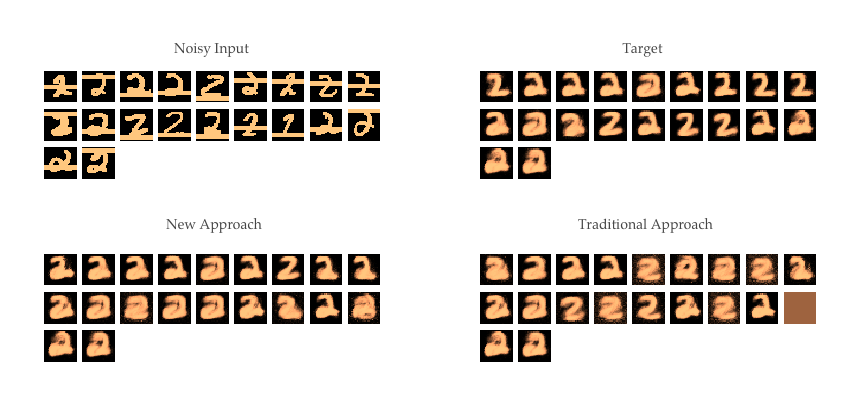
\includegraphics[width=1\textwidth]{Assets/Initial_Results}
% \caption[Initial results using new approach on noisy handwritten two images.]{Initial results using new approach on noisy handwritten two images. The input was 20 MNIST two digits with a random 4 pixel high bar composited. The new technique does not perform better by much over the dataset.  }
% \label{F:digit_example}
% \end{center}
% \end{figure}
%
%
% Another performance test carried out has been classification performance. The hypothesis being that the new approach should be able to generate a better representation despite having noisy training and test sets. The actual classification is deferred to an AI classifier that is trained on the hidden representations.
% Fig \ref{F:rbmClassification} shows a visual representation of this. The RBM is trained on some data, then a hidden representation and known labels are used to create a transformed training and test set which a perceptron or other classifier is then trained on. The better the classification performance the better representation the model has achieved.
% \begin{figure}[htbp]
% \begin{center}
% 	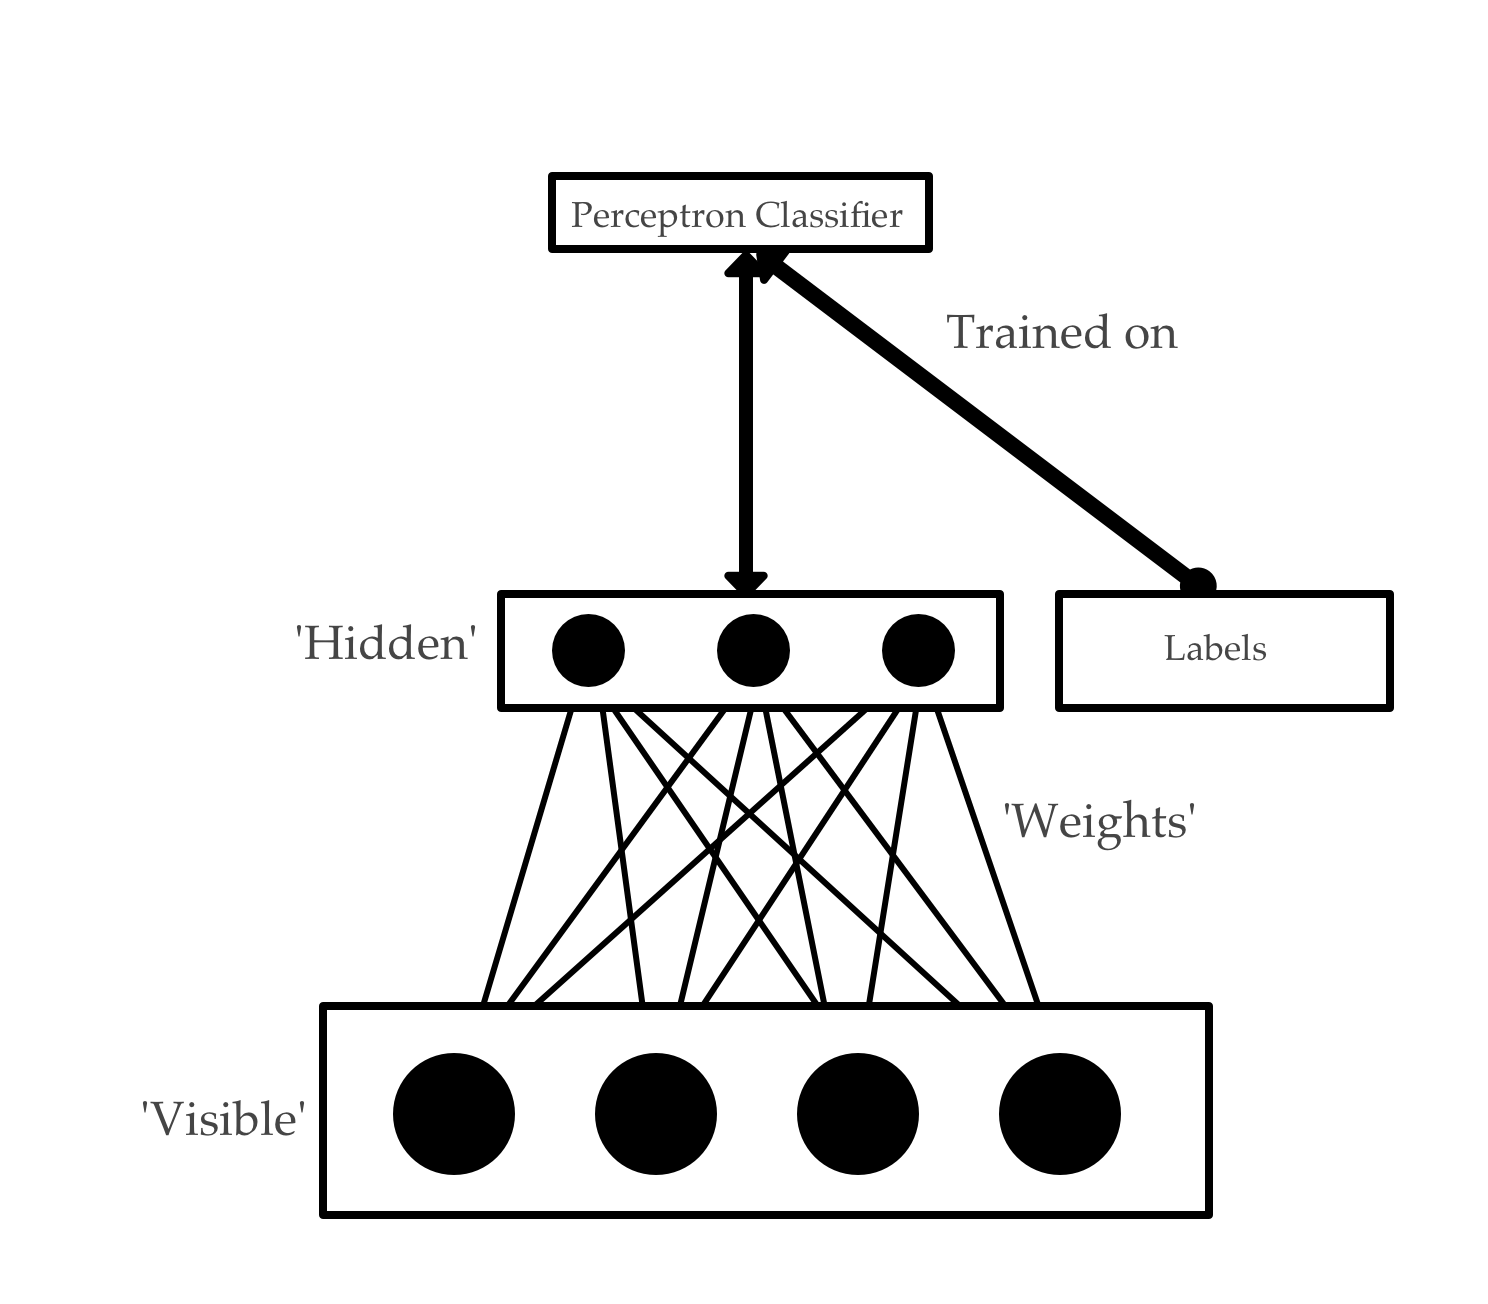
\includegraphics[width=0.7\textwidth]{Assets/RBMClassification}
% \caption[Figure demonstrating how classification can be applied using an RBM]{Figure demonstrating how classification can be applied using an RBM. }
% \label{F:rbmClassification}
% \end{center}
% \end{figure}
%
% \begin{figure}[htbp]
% \begin{center}
% 	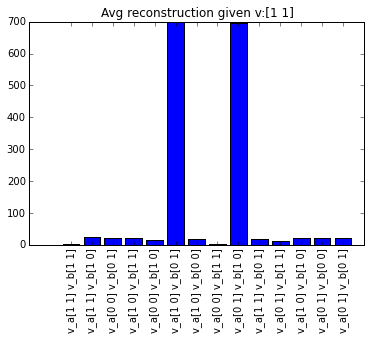
\includegraphics[width=0.7\textwidth]{Assets/yup}
% \caption{Figure showing the results of generating reconstructions using the new approach and two identical RBMs that can recognise a single pixel being on a time.}
% \label{F:twobit}
% \end{center}
% \end{figure}
%
% The non-outstanding results shown in \ref{F:digit_example} and the other digits, highlighted that some minimal test cases need to be satisfied before more complicated models like digits can be explored. The tests currently in place are not atomic enough.
%
% We arrived at the minimal test case, a two bit image, with binary pixels and a toy RBM model trained to understand one pixel being on at a time. This had the advantage of being able to be checked by hand and approximations of the correction could be explored in the minimal case. This is the  smallest case possible for them to actually work and as a result, more robust correction tests have been constructed.
%
% In the two bit scenario it is very easy to measure the performance of reconstructions, we would hope given an visible input of $ v = [1,1] $ that the new approach would most of the time result in reconstructions from the two models of $ v'_A = [1,0]$,  $v'_B = [0,1] $ and conversely $ v'_A = [0,1]$,  $v'_B = [1,0] $. Where $v'_A$ is the reconstruction generated, given $v$ from model A.
%
% The results of doing this in a two bit system, that is two hidden and two visible units resulted in the plot in fig \ref{F:twobit}. We see the most common reconstructions are those defined above. It is important to look at the reconstructions from both models holistically to ensure they are actually separating the sources. The figure shows the average of 1000 runs of the new approach, the two bit example making this many runs quite feasible with so few features.
%
%
% \section{Evaluation Planning}\label{S:evaluation}
%
% As the output of the project is essentially a series of reproducible performance results, it is important that the algorithm is sound in practice and matches what the theory describes. The validity of the results hinge on the confidence that the code does what it should. This precondition is enforced by unit and integration testing the system. The third party libraries in use for linear algebra (NumPy) and plotting (Matplotlib) are well tested and feature in other peer reviewed literature in the field of Machine Learning \cite{Millman:2011wp}.
%
% As touched on in the scope changes in section \ref{S:ScopeChanges} the evaluation phase of the project needs to be ongoing. The performance of the new approach needs to be checked at every point to ensure that cases where the new approach does and does not work can be pinpointed. It also makes tracking down what factors make it more or less effective easier.
% The actual approach to evaluation is touched on above, but it amounts to verifying if and when the new approach generates a better representation of a composite image versus that of the traditional approach.

%
% 

\chapter{Future Work}\label{C:Future Work}

Going forward it will be important to move from working with two bit images back up to larger images with non-toy models - i.e. the MNIST handwritten digit dataset.
An outcome of the next step is being able to train two RBMs from purely composite data. For instance, being able to train an RBM that learnt a representation of a digit and another of noise from only seeing digits combined with noise. If this is fruitful, it will amount to blind source separation.

It is worth noting that out of scope at the moment is using actual photos, as this would require significantly more computing power. The runtime of this new approach needs to be tested for correctness on smaller images before this can occur. Also this might require aligning the content images and potentially acquiring a larger image dataset. Working with datasets like MNIST where this has already been applied allows the focus to be on evaluating the new technique.

\begin{figure}
  \begin{center}
    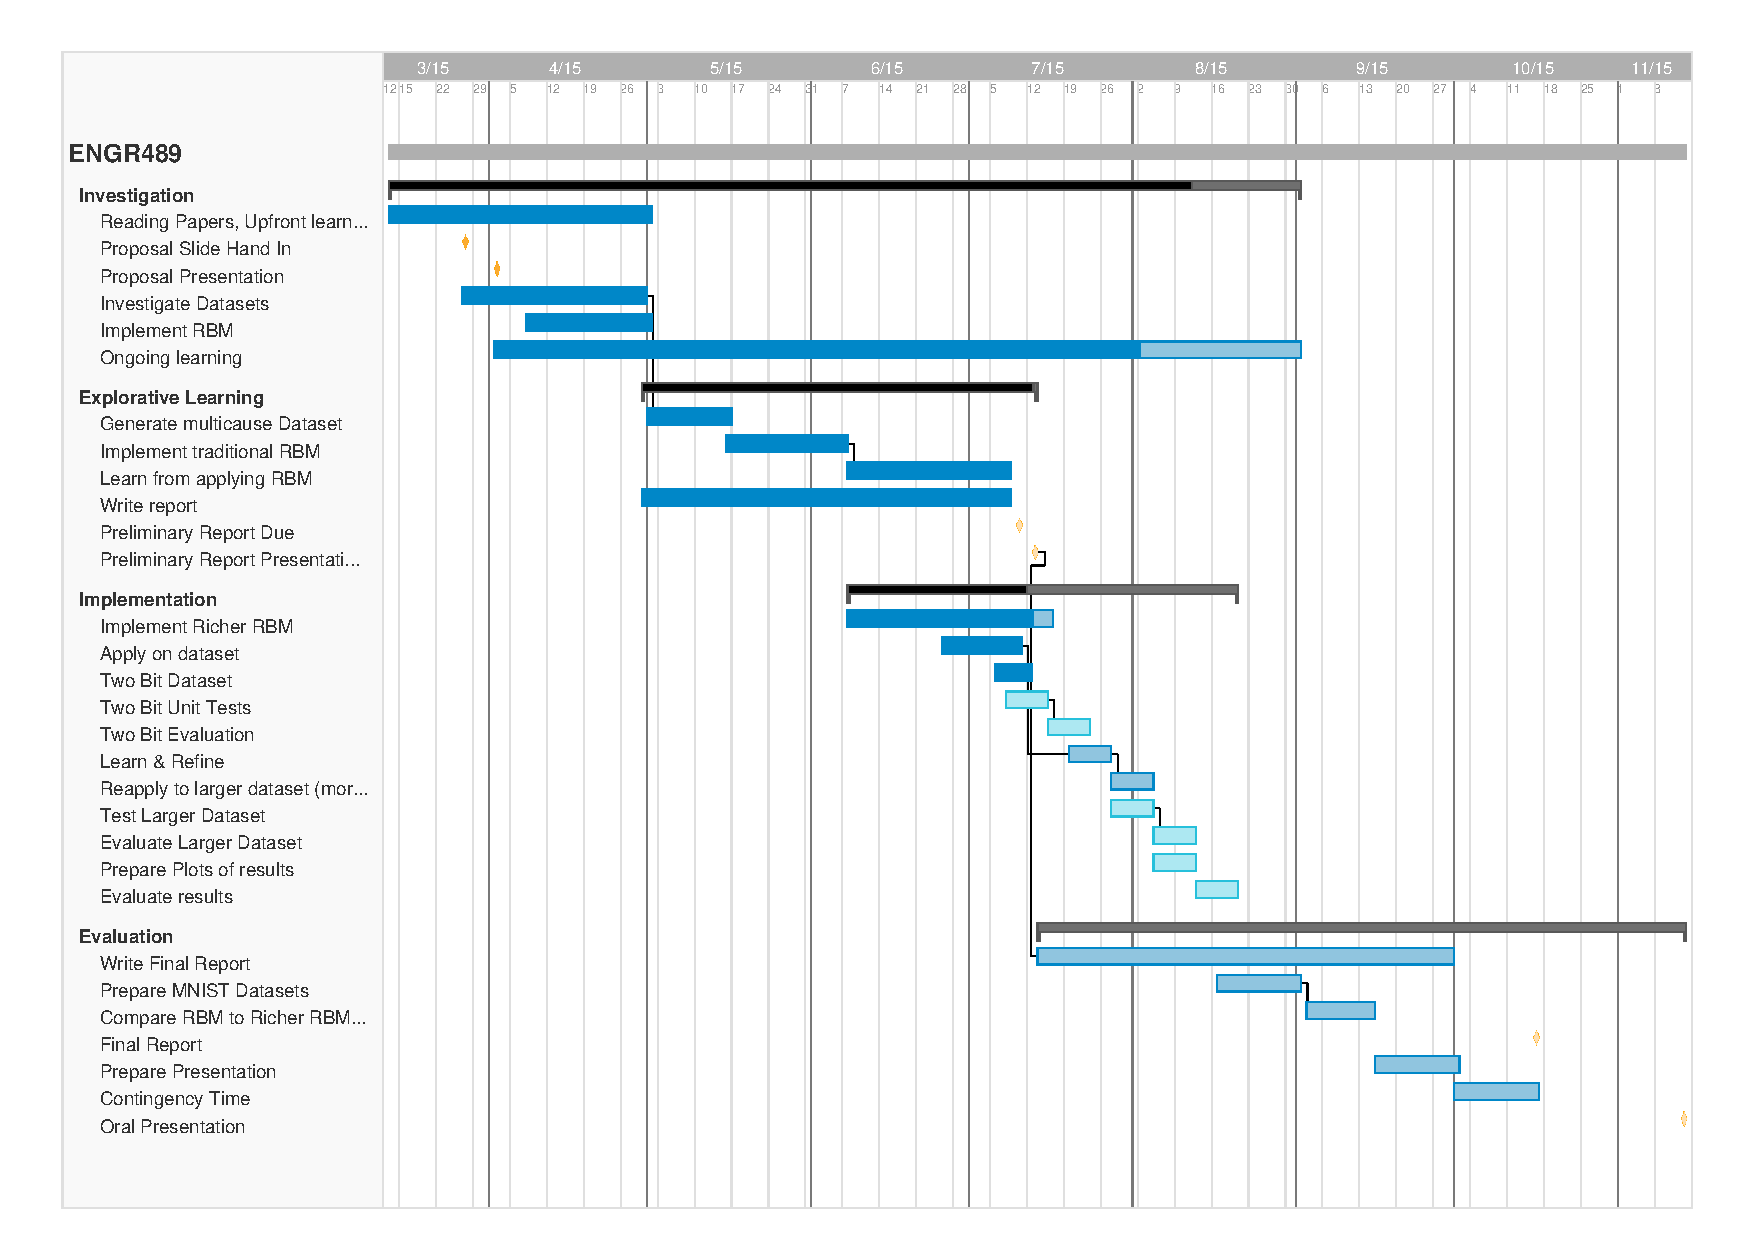
\includegraphics[width=1\textwidth]{Assets/gantt}
    \caption{Revised Gantt chart}
   \label{F:gantt}
   \end{center}
\end{figure}


\backmatter

\bibliographystyle{acm}
\bibliography{sample}

\end{document}
